\documentclass[reprint,amsmath,amssymb,aps]{revtex4-1}

\usepackage{graphicx}
\usepackage{natbib}
\usepackage{amsmath}
\usepackage{gensymb}
\usepackage{enumerate}
\usepackage{varwidth}
\usepackage{float}
\usepackage{nonfloat}
% \usepackage{afterpage}
\usepackage[usenames, dvipsnames]{color}
\newcommand{\note}[1]{\noindent \textbf{\textit{\textcolor{Red}{#1}}}}

\newcommand\Ra{\mathrm{Ra}}
\newcommand\Pran{\mathrm{Pr}}
\newcommand\Rac{\mathrm{Ra}_{\mathrm{c}}}
\newcommand\Ek{\mathrm{Ek}}
\newcommand\Ro{\mathrm{Ro}}
\newcommand\Nu{\mathrm{Nu}}
\newcommand\Sc{\mathrm{Sc}}

\newcommand\eps{\varepsilon}
\renewcommand\L {\mathcal{L}}

\newcommand{\n}{\\ \nonumber \\ }
\newcommand{\nn}{\nonumber}
\newcommand{\nnn}{\\ \nonumber \\ \nonumber}

\newcommand\ie{\textit{i.e.},~}
\newcommand\eg{\textit{e.g.},~}
\newcommand{\omicron}{o}

\newcommand{\pd}[1]{\partial_{#1}}
\renewcommand{\vec}[1]{\boldsymbol{#1}}
\newcommand{\M}[1]{\mathbf{#1}}
\newcommand{\grad}{\vec{\nabla}}
\newcommand{\cross}{\vec{\times}}
\newcommand{\laplacian}{\nabla^2}

\newcommand{\sump}[2]{\sideset{}{'}\sum_{{#1}=0}^{#2}}

\newcommand{\eq}[1]{eq.~(\ref{#1})}
\newcommand{\eqs}[2]{eqs.~(\ref{#1})~\&~(\ref{#2})}
\newcommand{\eqss}[2]{eqs.~(\ref{#1})--(\ref{#2})}

\newcommand{\Eq}[1]{Eq.~(\ref{#1})}
\newcommand{\Eqs}[2]{Eqs.~(\ref{#1})~\&~(\ref{#2})}
\newcommand{\Eqss}[2]{Eqs.~(\ref{#1})--(\ref{#2})}

\newcommand{\fig}[1]{Fig.~(\ref{#1})}
\newcommand{\figs}[2]{Figs.~(\ref{#1})~\&~(\ref{#2})}
\newcommand{\T}{{\cal T}}
\newcommand{\Z}{{\cal Z}}

\bibliographystyle{apsrev4-1}

\makeatletter
\let\Hy@backout\@gobble
\makeatother

\newcommand*{\GtrSim}{\smallrel\gtrsim}

\makeatletter
\newcommand*{\smallrel}[2][.8]{%
  \mathrel{\mathpalette{\smallrel@{#1}}{#2}}%
}
\newcommand*{\smallrel@}[3]{%
  % #1: scale factor
  % #2: math style
  % #3: symbol
  \sbox0{$#2\vcenter{}$}%
  \dimen@=\ht0 %
  \raise\dimen@\hbox{%
    \scalebox{#1}{%
      \raise-\dimen@\hbox{$#2#3\m@th$}%
    }%
  }%
}
\makeatother


\begin{document}

\title{Marginally-Stable Thermal Equilibria of Rayleigh-Bénard Convection}

\author{Liam O'Connor$^1$}
\author{Daniel Lecoanet$^{1, 2}$}
\author{Evan Anders$^2$}
\affiliation{%
$^1$Department of Engineering Sciences and Applied Mathematics, Northwestern University, Evanston, IL 60208 USA}
\affiliation{%
$^2$Center for Interdisciplinary Exploration and Research in Astrophysics, Northwestern University, Evanston, IL, 60201 USA}

\begin{abstract}
Natural convection is ubiquitous throughout the physical sciences and engineering, yet many of its important properties remain elusive -- particularly in the large Rayleigh number regime.
In this investigation, we derive and solve a quasilinear form of the Boussinesq Rayleigh-B\'enard equations. 
Eigenfunction amplitudes are obtained by requiring marginal-stability. We obtain symmetric thermally-equilibrated solutions and analyze their properties. 
Solutions to the quasilinear problem differ from statistically-steady 2-dimensional Rayleigh-Be\'nard convection simulation data, having thinner boundary layers and larger Nusselt numbers $\Nu$ which scale like $\Nu \sim Ra^{1/3}$. 
We initialize 2-dimensional simulations with solutions to the quasilinear problem; they do not undergo a convective transient period and are kinetically exaggerated.
\end{abstract}


\maketitle

\section{Introduction}
Rayleigh-B\'enard convection plays a foundational role in large-scale astrophysical and geophysical settings.
Buoyancy-driven convection regulates heat transfer and often gives way to violently turbulent flows, thereby dominating the large-scale behaviors and fueling small-scale processes \cite{Couston} in important systems.

Aggressive convection, which is associated with large Rayleigh numbers $Ra$, is difficult to simulate. 
State of the art convection simulations performed by \cite{Zhu} have reached $Ra = 10^{14}$ but estimates for stars are $Ra \sim 10^{20}$ \cite{Ossendrijver}. 
The scaling behavior of the Nusselt number $\Nu$ (nondimensionalized heat transfer) in the highly turbulent ultimate regime is of particular interest.
There exists a substantial body of work pertaining to this specific topic with no general consensus \cite{Malkus}, \cite{Kraichnan} \cite{Spiegel}, \cite{Castaing}, \cite{Grossman}, \cite{Ahlers}. 

Reduced models are particularly useful in this context because they allow us to study the problem with relatively low expense. 
Much of the published work on this topic relates to unstable coherent solutions \cite{Waleffe}, \cite{Sondak}, \cite{Wen}, \cite{chini_cells}. 
Simulations and analysis performed by \cite{Yalniz} and \cite{Cvitanovic} suggest that chaotic solution trajectories can be modelled as a Markov chain whose long-term behavior is given by the time-weighted-average of a finite set of unstable coherent solutions. Should that be the case, it is crucial that we discover and classify such states.

In \cite{Chini_sw}, researchers develop and solve a quasilinear formulation of the Navier-Stokes equations via multi-scale asymptotic arguments. This is realized by defining a mean state which hypothetically evolves on a slow time-scale. An analytic expression for the first-order perturbations' amplitude is found by deriving a solvability condition of the second-order perturbations and integrating over the domain spatially. 
We seek to solve the Boussinesq Rayleigh–Bénard convection equations using an analogous strategy. 
The application of this procedure yields time-invariant solutions to the quasilinear problem with a range of expected and unexpected features. 

\section{Model Setup}\label{sec:model}
We begin with the non-dimensionalized Boussinesq approximation for Rayleigh-Bénard Convection. 
The domain is 2-dimensional rectangular and horizontally periodic with spatial dimensions $0 < x < 4$ and $-1/2 < z < 1/2$. 
The fluid of interest is constrained between two planar boundaries at $z = -1/2$ and $z = 1/2$ with fixed temperatures $1$ and $0$ respectively. 
At both boundaries we specify impenetrable, no-slip conditions, such that the velocity $\mathbf{u} = u \hat{x} + w \hat{z} = \mathbf{0}$ at $z = \pm 1/2$. 
The equations of motion are then given by
\begin{align}
    \nabla \cdot \mathbf{u} &= 0 \label{EQ:motion1}\\
    \frac{\partial \mathbf{u}}{\partial t} + \mathbf{u} \cdot \nabla \mathbf{u} &= - \nabla p + T \hat{z} + \mathcal{R} \nabla^2 \mathbf{u} \label{EQ:motion2}\\
    \frac{\partial T}{\partial t} + \mathbf{u} \cdot \nabla T &= \mathcal{P} \nabla^2 T \label{EQ:motion3}
\end{align}
where $p$ is pressure and $T$ is temperature. 
For completeness, we specify a final boundary condition $p = p_0$ at $z = \pm 1/2$. 
Any system of this form can be characterized by its dimensionless Rayleigh number $Ra = \frac{g\alpha L^3 \Delta T}{\nu \kappa}$ and Prandtl number $Pr = \frac{\nu}{\kappa}$, where $g, \, \alpha, \, L, \, \Delta T, \nu, \kappa$ are the gravitational acceleration, coefficient of thermal expansion, domain height, boundary temperature difference, kinematic viscosity, and thermal diffusivity respectively. 
\begin{equation}
\mathcal{R} = \sqrt{\frac{Pr}{Ra}}, \qquad \mathcal{P} = \frac{1}{\sqrt{Pr Ra}}.
\end{equation}

To derive the linearized system, we posit that each field can be represented as the sum of a mean profile (denoted by $\bar{\cdot } \;$) and a perturbation function (denoted by $\cdot'$).
\begin{align}
    \mathbf{u}(x, z, t) &= \mathbf{u'}(x, z, t) \label{EQ:reynolds_dc_u}\\
    &= u'(x, z, t)\hat{x} + w'(x, z, t)\hat{z} \\
    T(x, z, t) &= \bar{T}(z) + T'(x, z, t) \label{EQ:reynolds_dc_T}\\
    p(x, z, t) &= \bar{p}(z) + p'(x, z, t).
\end{align}
Upon substitution, we equate terms which scale linearly with the perturbations, yielding the linearized stability equations
\begin{align}
    \nabla \cdot \mathbf{u'} &= 0 \label{EQ:linear1}\\
    \frac{\partial\mathbf{u'}}{\partial t} &= - \nabla p' + T'\hat{z} + \mathcal{R} \nabla^2 \mathbf{u'} \label{EQ:linear2}\\
    \frac{\partial T'}{\partial t} + \frac{\partial \bar{T}}{\partial z} w' &= \mathcal{P} \nabla^2 T' \label{EQ:linear3}
\end{align}
with Dirichlet boundary conditions 
\begin{equation}
    T'|_{z = \pm \frac{1}{2}} = 0, \quad u'|_{z = \pm \frac{1}{2}} = 0, \quad p'|_{z = \pm \frac{1}{2}} = 0.
\end{equation}
In 1916, Lord Rayleigh observed that (\ref{EQ:linear1}) and (\ref{EQ:linear3}) can be manipulated into a separable form with generalized solutions
\begin{align}
    w'(x, z, t) &= W(z) \, e^{i(k_xx-st)} \label{EQ:normal_modes1}\\ 
    u'(x, z, t) &= U(z) \, e^{i(k_xx-st)} \label{EQ:normal_modes2}\\ 
    T'(x, z, t) &= \theta(z) \, e^{i(k_xx-st)} \label{EQ:normal_modes3}\\ 
    p'(x, z, t) &= P(z) \, e^{i(k_xx-st)}\label{EQ:normal_modes4}
\end{align}
where $s = \sigma + i\omega$ and $k_x$ is constrained, by periodicity, to the countably infinite set (spectrum) of wavenumbers
\begin{align}
    k_x \in \big\{\frac{n\pi}{2} \, \big| \, n \in \mathbb{N}\big\}.
\end{align}
For each $k_x$, we can assess the stability of the perturbations by solving for the eigenvalue $s$, whose imaginary component $\omega$ plays the role of an exponential growth rate. 
Solution yields a finite set of eigenvalues, among which, that with maximum $\omega$ is assumed to be dominant. 
Positive eigenvalues indicate that the system is unstable to small disturbances of wavenumber $k_x$, while negative eigenvalues indicate stability. 
A complete linear stability analysis requires solution over the full spectrum of wavenumbers. 
The prototypical case is used to demonstrate that the critical Rayleigh number $Ra_c = 1708$ when $\frac{\partial \bar{T}}{\partial z} = -1$.

For this investigation, we allow $\bar{T}$ to vary in $z$ and $t$. Substituting (\ref{EQ:reynolds_dc_T}) into (\ref{EQ:motion3}) yields
\begin{align}
    \frac{\partial \bar{T}}{\partial t} + \mathbf{u}' \cdot \nabla T' + \frac{\partial T'}{\partial t} + \frac{\partial \bar{T}}{\partial z} w' = \mathcal{P} \nabla^2 T' + \mathcal{P} \nabla^2 \bar{T}.
    \label{EQ:T't_xz}
\end{align}
Subtracting (\ref{EQ:linear3}) from (\ref{EQ:T't_xz}) eliminates several terms. 
We can replace the advective term $\mathbf{u}' \cdot \nabla T'$ with $\grad \cdot (\mathbf{u}'T')$ due to (\ref{EQ:linear1}). 
Taking the horizontal average of (\ref{EQ:T't_xz}), this advective term can be reduced to
\begin{align}
    \frac{1}{4}\int_0^4 \grad \cdot (\mathbf{u}'T') dx &= \frac{\partial }{\partial z}  \langle w'T' \rangle
\end{align}
where $\langle \cdot \rangle$ denotes the horizontal average. 
The remaining terms in (\ref{EQ:T't_xz}) are unaffected as they are independent of $x$. 
The eigenfunctions $W(z),\, U(z),\, \theta(z),$ and $P(z)$ do not admit any natural normalization, as (\ref{EQ:linear1}) -- (\ref{EQ:linear3}) and their subsequent forms are linear with respect to the perturbations. 
For completeness, we provide the normalization 
\begin{equation}
    \int_{-\frac{1}{2}}^{\frac{1}{2}} \big| \theta (z) \big| dz = 1
\end{equation}
and assign each perturbation a yet-unknown amplitude $A \in \mathbb{R}$, thereby allowing us to reduce (\ref{EQ:T't_xz}) to the initial value problem (IVP)
\begin{equation}
    \frac{\partial \bar{T}}{\partial t} + A^2 \langle w'T' \rangle = \mathcal{P}  \frac{\partial^2 \bar{T}}{\partial z^2}, \label{EQ:T0_IVP}
\end{equation}
upon which the remainder of this investigation is centered. 
It is important to keep in mind that the forcing term $\langle w'T' \rangle$ is obtained by solving an eigenvalue problem (EVP) which itself involves $\frac{\partial \bar{T}}{\partial z}$. 
We also assume this term is composed of eigenfunctions belonging to the dominant mode. 

\section{Perturbation Evolution}
Solving the linearized system (\ref{EQ:linear1}) -- (\ref{EQ:linear3}) does not yield $A^2$. 
To evolve $\bar{T}$ numerically, we assume the perturbations and mean quantities depend on different time-scales, as in \cite{Chini_sw}. On the fast time-scale, stable modes will decay and unstable modes will act according to (\ref{EQ:T0_IVP}). 
We make the ansatz that only marginally stable modes will affect $\bar{T}$ on long time-scales
\begin{equation}
    \max_{k_x} \{ \omega \} = 0
\end{equation}
thereby constraining $A^2$ at each timestep.

For various $Ra$ and fixed $Pr = 1$, we seek symmetric, marginally-stable temperature profiles $\bar{T}_{eq}(z)$ which are thermally equilibrated, thereby satisfying $\frac{\partial \bar{T}_{eq}}{\partial t} = 0$ according to (\ref{EQ:T0_IVP}). 
We employ the \texttt{Dedalus} pseudo-spectral python framework to solve the EVP outlined in Section \ref{sec:model} as well as the IVP (\ref{EQ:T0_IVP}) by representing each field with a dealiased Chebyshev polynomial basis. 
The necessary number of basis functions varies, as eigenfunctions and temperature profiles associated with large Rayleigh numbers admit increasingly small-scale features. 
We supplement \texttt{Dedalus} with the \texttt{Eigentools} package to obtain the eigenfunctions in (\ref{EQ:T0_IVP}).

To find an equilibrated profile, we begin with a marginally-stable initial profile $\bar{T}_0(z)$ whose construction is outlined in \ref{sec:initial_profile}. 
We seek to evolve $\bar{T}_0(z)$ into a new marginally-stable profile $\bar{T}_1(z)$ according to (\ref{EQ:T0_IVP}) using forward-Euler. 
This generally involves a unique and unknown value $A^2 > 0$. 
Our method of finding $A^2$ is best illustrated through example.

\begin{figure}
    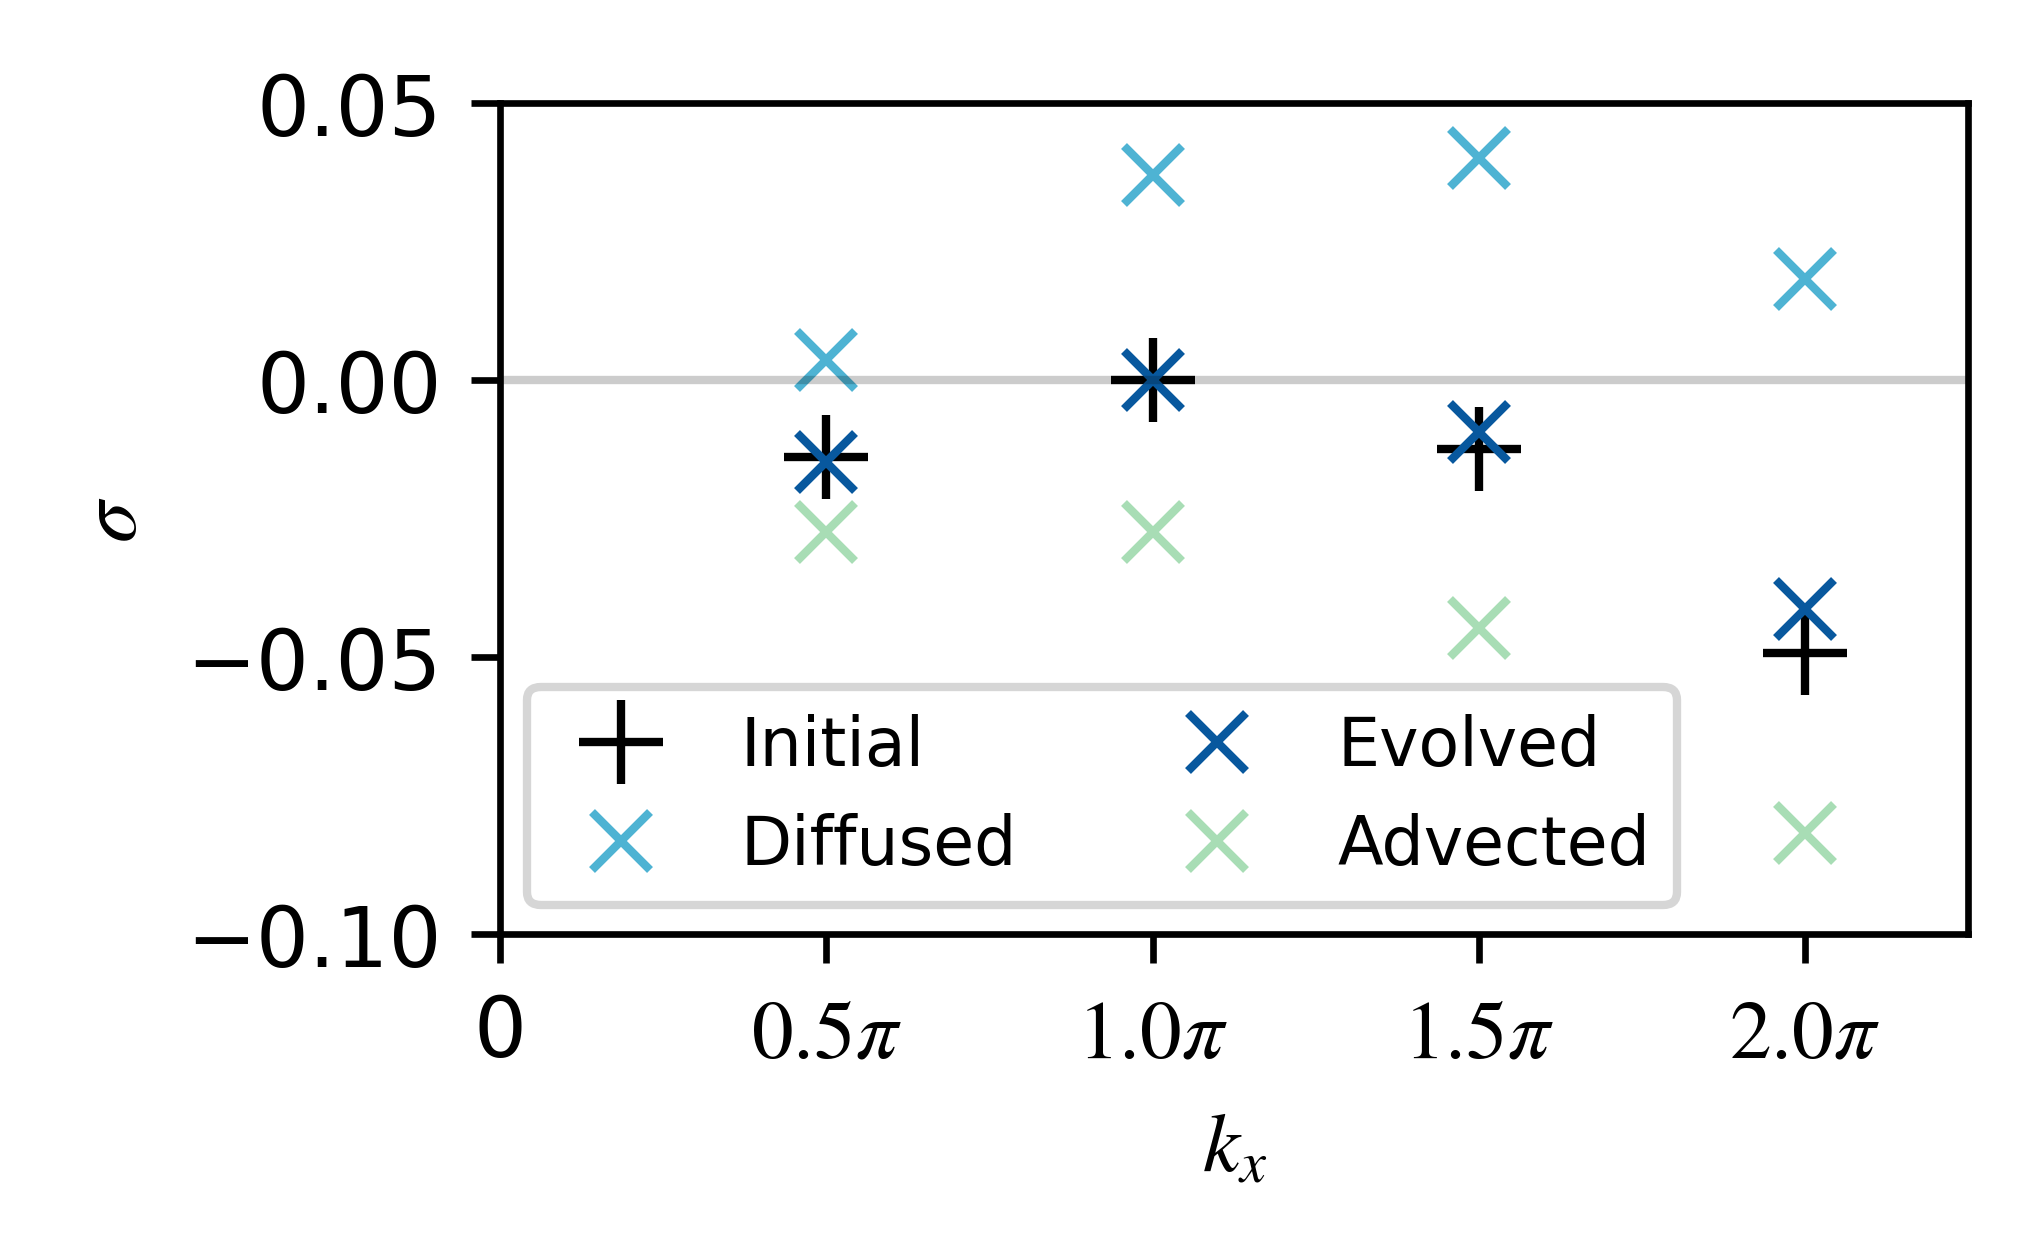
\includegraphics[width=3.4in]{EV_spectrum_ol.png}
    \caption{Eigenvalue spectra for $Ra = 10^5$. The spectrum of a marginally-stable mean temperature profile $\bar{T}_0$ (shown in black) has a maximum eigenvalue of 0. 
    Given a small fixed timestep $\Delta t$, diffusion destabilizes the system, increasing its eigenvalues (shown in blue). 
    Advection tends to stabilize the system, decreasing its eigenvalues (shown in red). 
    It follows that there exists some proportion ($A^2$) of these two terms which yields a new marginally-stable mean temperature profile $\bar{T}_1$, whose spectrum is shown in green.}
    \label{fig:iteration_spectra} 
\end{figure}

An iteration is performed as follows: diffusing a marginally-stable temperature profile $\bar{T}_0$ tends to increase its eigenvalues. 
Ignoring the diffusive term and evolving according to advection tends the stabilize the system. The appropriate amplitude $A^2$ can then be approximated by
\begin{equation}
    A^2 \sim -\frac{\omega_{\rm{diff}}}{\omega_{\rm{adv}}}
\end{equation}
where $\omega_{\rm{diff}}$ and $\omega_{\rm{adv}}$ refer to the diffused and advected eigenvalues of the initially marginal mode (corresponding to the blue and red points respectively at $k_x = \pi$ in Figure \ref{fig:iteration_spectra}). 
$\bar{T}_0$ is then evolved according to (\ref{EQ:T0_IVP}) and another eigenvalue solve is performed. 
Given a fixed timestep $\Delta t$, we assume the dominant eigenvalue can be described by a continuous function $\omega_{\rm{max}} (A^2)$ which is locally differentiable. 
Newton's method is used to find an amplitude which meets our marginal stability tolerance criterion $|\omega_{\rm{max}} (A^2)| \leq 10^{-9}$. 
The dominant mode is not fixed; an iteration can facilitate the transfer of marginal-stability from one mode to another. 
In section \ref{sec:multiple_modes} we specify procedures for the treatment of multiple simultaneously marginal modes.

\subsection{Treatment of multiple marginally-stable modes} \label{sec:multiple_modes}
In most cases, we eventually encounter eigenvalue spectra with multiple simultaneously marginal modes. If ignored, we are forced to reduce the timestep and allow the modes to alternate. Instead, we generalize the advective term in (\ref{EQ:T0_IVP}) to accommodate $N$ simultaneously marginal modes
\begin{equation}
    A^2 \langle w' b' \rangle = \sum_{n = 1}^{N} A^2_{n} \langle w' b' \rangle_{n}
\end{equation}
where  $\langle w' b' \rangle_{n}$ is composed of perturbations associated with $k_x = \frac{n\pi}{2}$. 
There are now $N$ amplitudes to solve for and $N$ eigenvalues to keep marginally-stable. 
In general, we expect a function $\mathbf{\omega} \, : \, \mathbb{R}^N \to  \mathbb{R}^N$ to have isolated roots (should they exist). 
We employ Broyden's method for root-finding in multi-dimensional functions whose derivatives are not explicitly known. 
Difficulty arises when transitioning between different numbers of marginal modes. 
Here we rely on $A^2 > 0$ by asserting that a mode which is \textit{close enough} to marginal-stability can be included in the iteration provided that its respective amplitude is positive. 
Should we converge upon a negative amplitude, that mode is discarded and the iteration is repeated. 
In general we find that no other obvious course of action yields equilibria.

\section{Properties of Thermally Equilibrated States}\label{sec:properties}
Thermally equilibrated states of this kind are solutions to a particular quasilinear form of the Rayleigh-B\'enard convection equations. 
For this investigation, we calculate solutions for $Ra$ in the range $10^5 - 10^9$. 
Solutions are symmetric about $z = 0$ by construction. 
This, combined with the fact that we did initialize a mean horizontal flow implies the absence of any nonzero horizontal velocity perturbations, as is the case in \cite{Waleffe}. 

Figure \ref{fig:T0_profiles} gives temperature profiles for $Ra = 10^8$ where the initial profile, given by (\ref{EQ:T0}), is employed at iteration 0; the equilibrated profile corresponds to the thermally relaxed state; and the simulation profile is obtained by performing a nonlinear simulation of (\ref{EQ:motion1})-(\ref{EQ:motion3}) with \texttt{Dedalus}, followed by horizontal and time averaging. 
The simulation curve is more diffuse than the equilibrated curve, which in turn, is more diffuse than the initial curve. 
Performing an eigenvalue solve by setting $\bar{T}$ equal to the simulation profile yields positive eigenvalues. 
Comprehensively, this suggests that thermally-equilibrated states might maximize boundary layer thickness, while subject to the marginal stability constraint.

The most resilient and unexpected feature of thermally equilibrated mean temperature profiles are the pronounced dips adjacent to the boundary layers. 
These dips appear in every solution, regardless of $Ra$. 
Physically, they correspond to thin layers in which the temperature gradient reverses, contradicting a hypothesis of \cite{Malkus}. 
This counter-diffusion, which opposes overall heat transfer, is overcome by the coinciding advective flux, shown in Figure \ref{fig:flux}. 
\begin{figure}
    \centering
    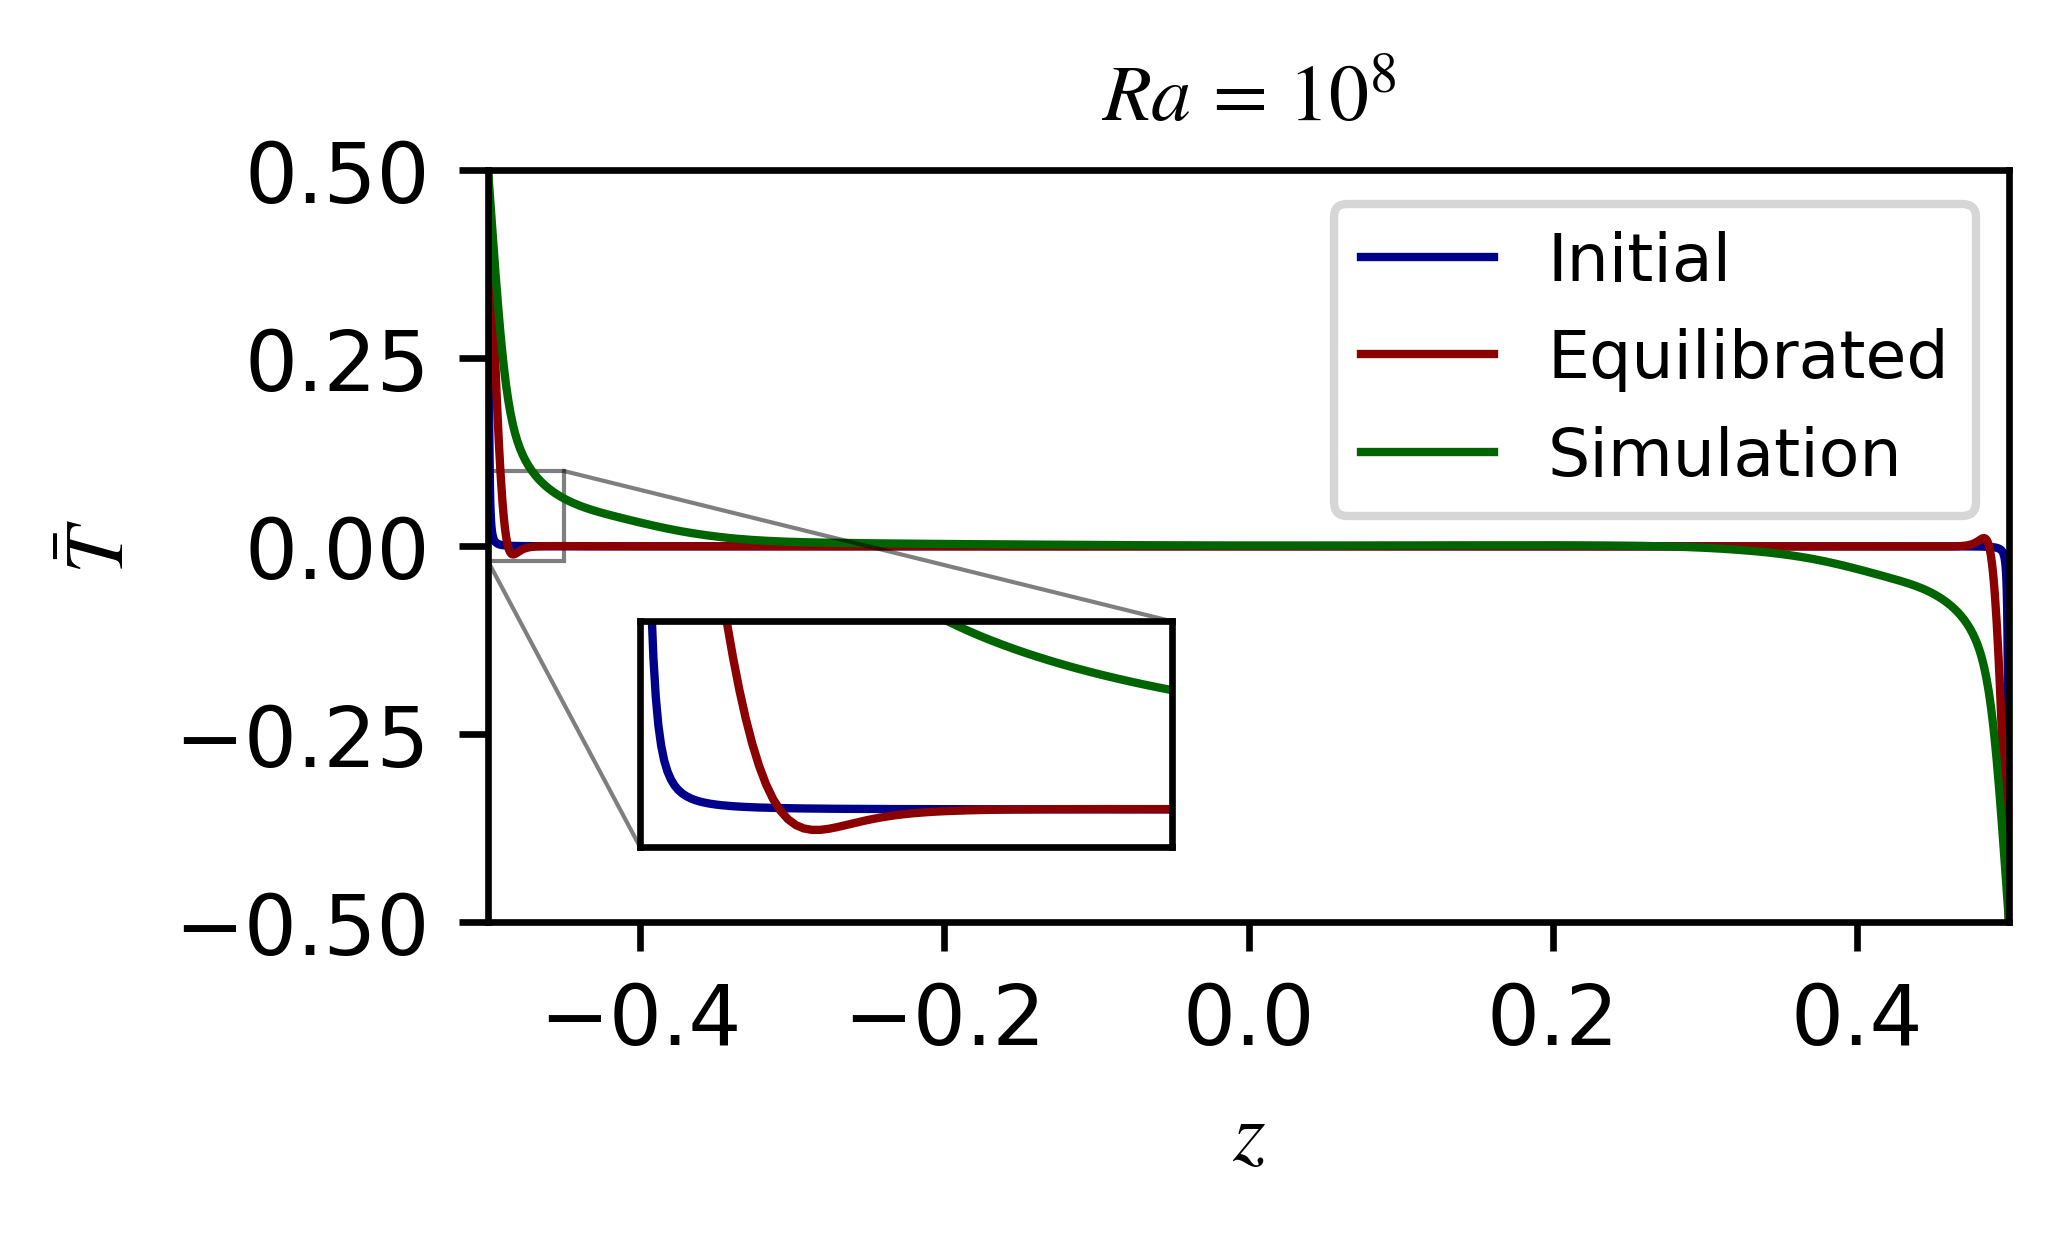
\includegraphics[width=3.4in]{T_profs_na.png}
    \caption{mean temperature profiles $\bar{T}$ for $Ra = 10^8$. 
    The initial profile is given by (\ref{EQ:T0}). 
    The equilibrated curve refers to the mean temperature profile of the marginally-stable thermally-equilibrated state. 
    The simulation profile is obtained by performing a 2-dimensional nonlinear simulation with \texttt{Dedalus} until thermal and kinetic relaxation. 
    The simulation temperature data are horizontally- and time-averaged. 
    The initial, equilibrated, and simulation profiles have increasingly relaxed boundary regions (respectively). 
    The equilibrated profile exhibits prominent dips, nested alongside the boundary regions. 
    The purpose of this feature is not well understood.}
    \label{fig:T0_profiles}
\end{figure}
\begin{figure}
    \centering
    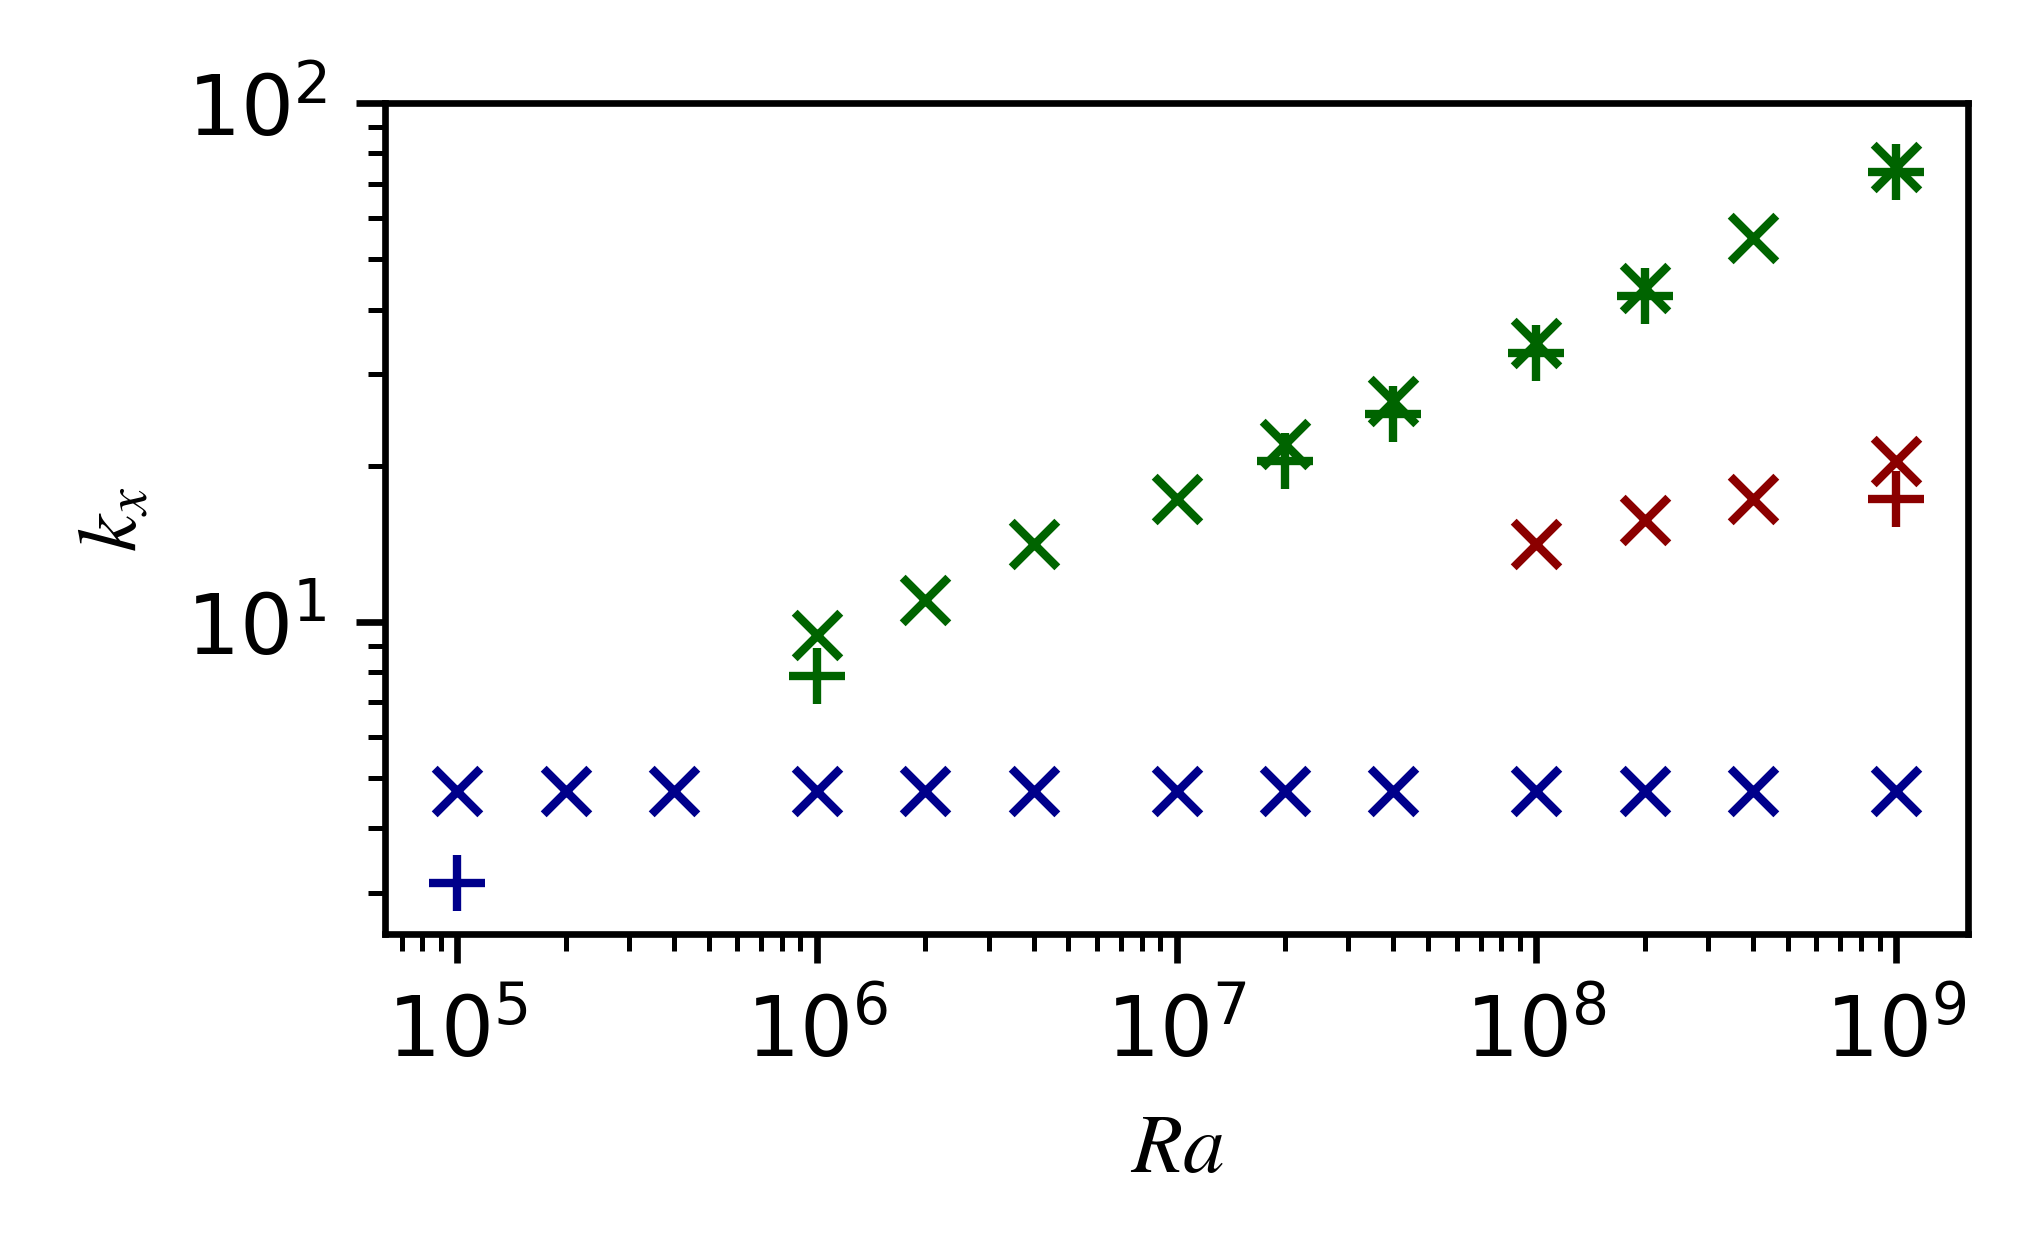
\includegraphics[width=3.4in]{kx_m_ra1.png}
    \caption{Wavenumbers of marginally-stable modes of thermally equilibrated states. 
    Markers are color-coded according to their adjacent local maxima index in the eigenvalue spectrum. 
    For example, the spectrum corresponding to $Ra = 10^5$ has marginal wavenumbers $k_x = \pi, \, 1.5\pi$ adjacent to a presumed local maximum between these two allowed values. 
    The $Ra = 10^9$ spectrum, shown in lower right corner of Figure \ref{fig:flux}, has three presumed local maxima, with a single marginal mode adjacent to the first maximum ($k_x = 1.5\pi$), two marginal modes adjacent to the second maximum ($k_x = 6\pi, \, 6.5\pi$), and two marginal modes adjacent to the third maximum ($k_x = 23.5\pi, \, 24\pi$). 
    The largest wavenumbers of the green branch obey a power-law relationship with $Ra$}
    \label{fig:kx_marginals}
\end{figure}
\begin{figure*}
    \centering
    \begin{tabular}{@{}c@{}}
        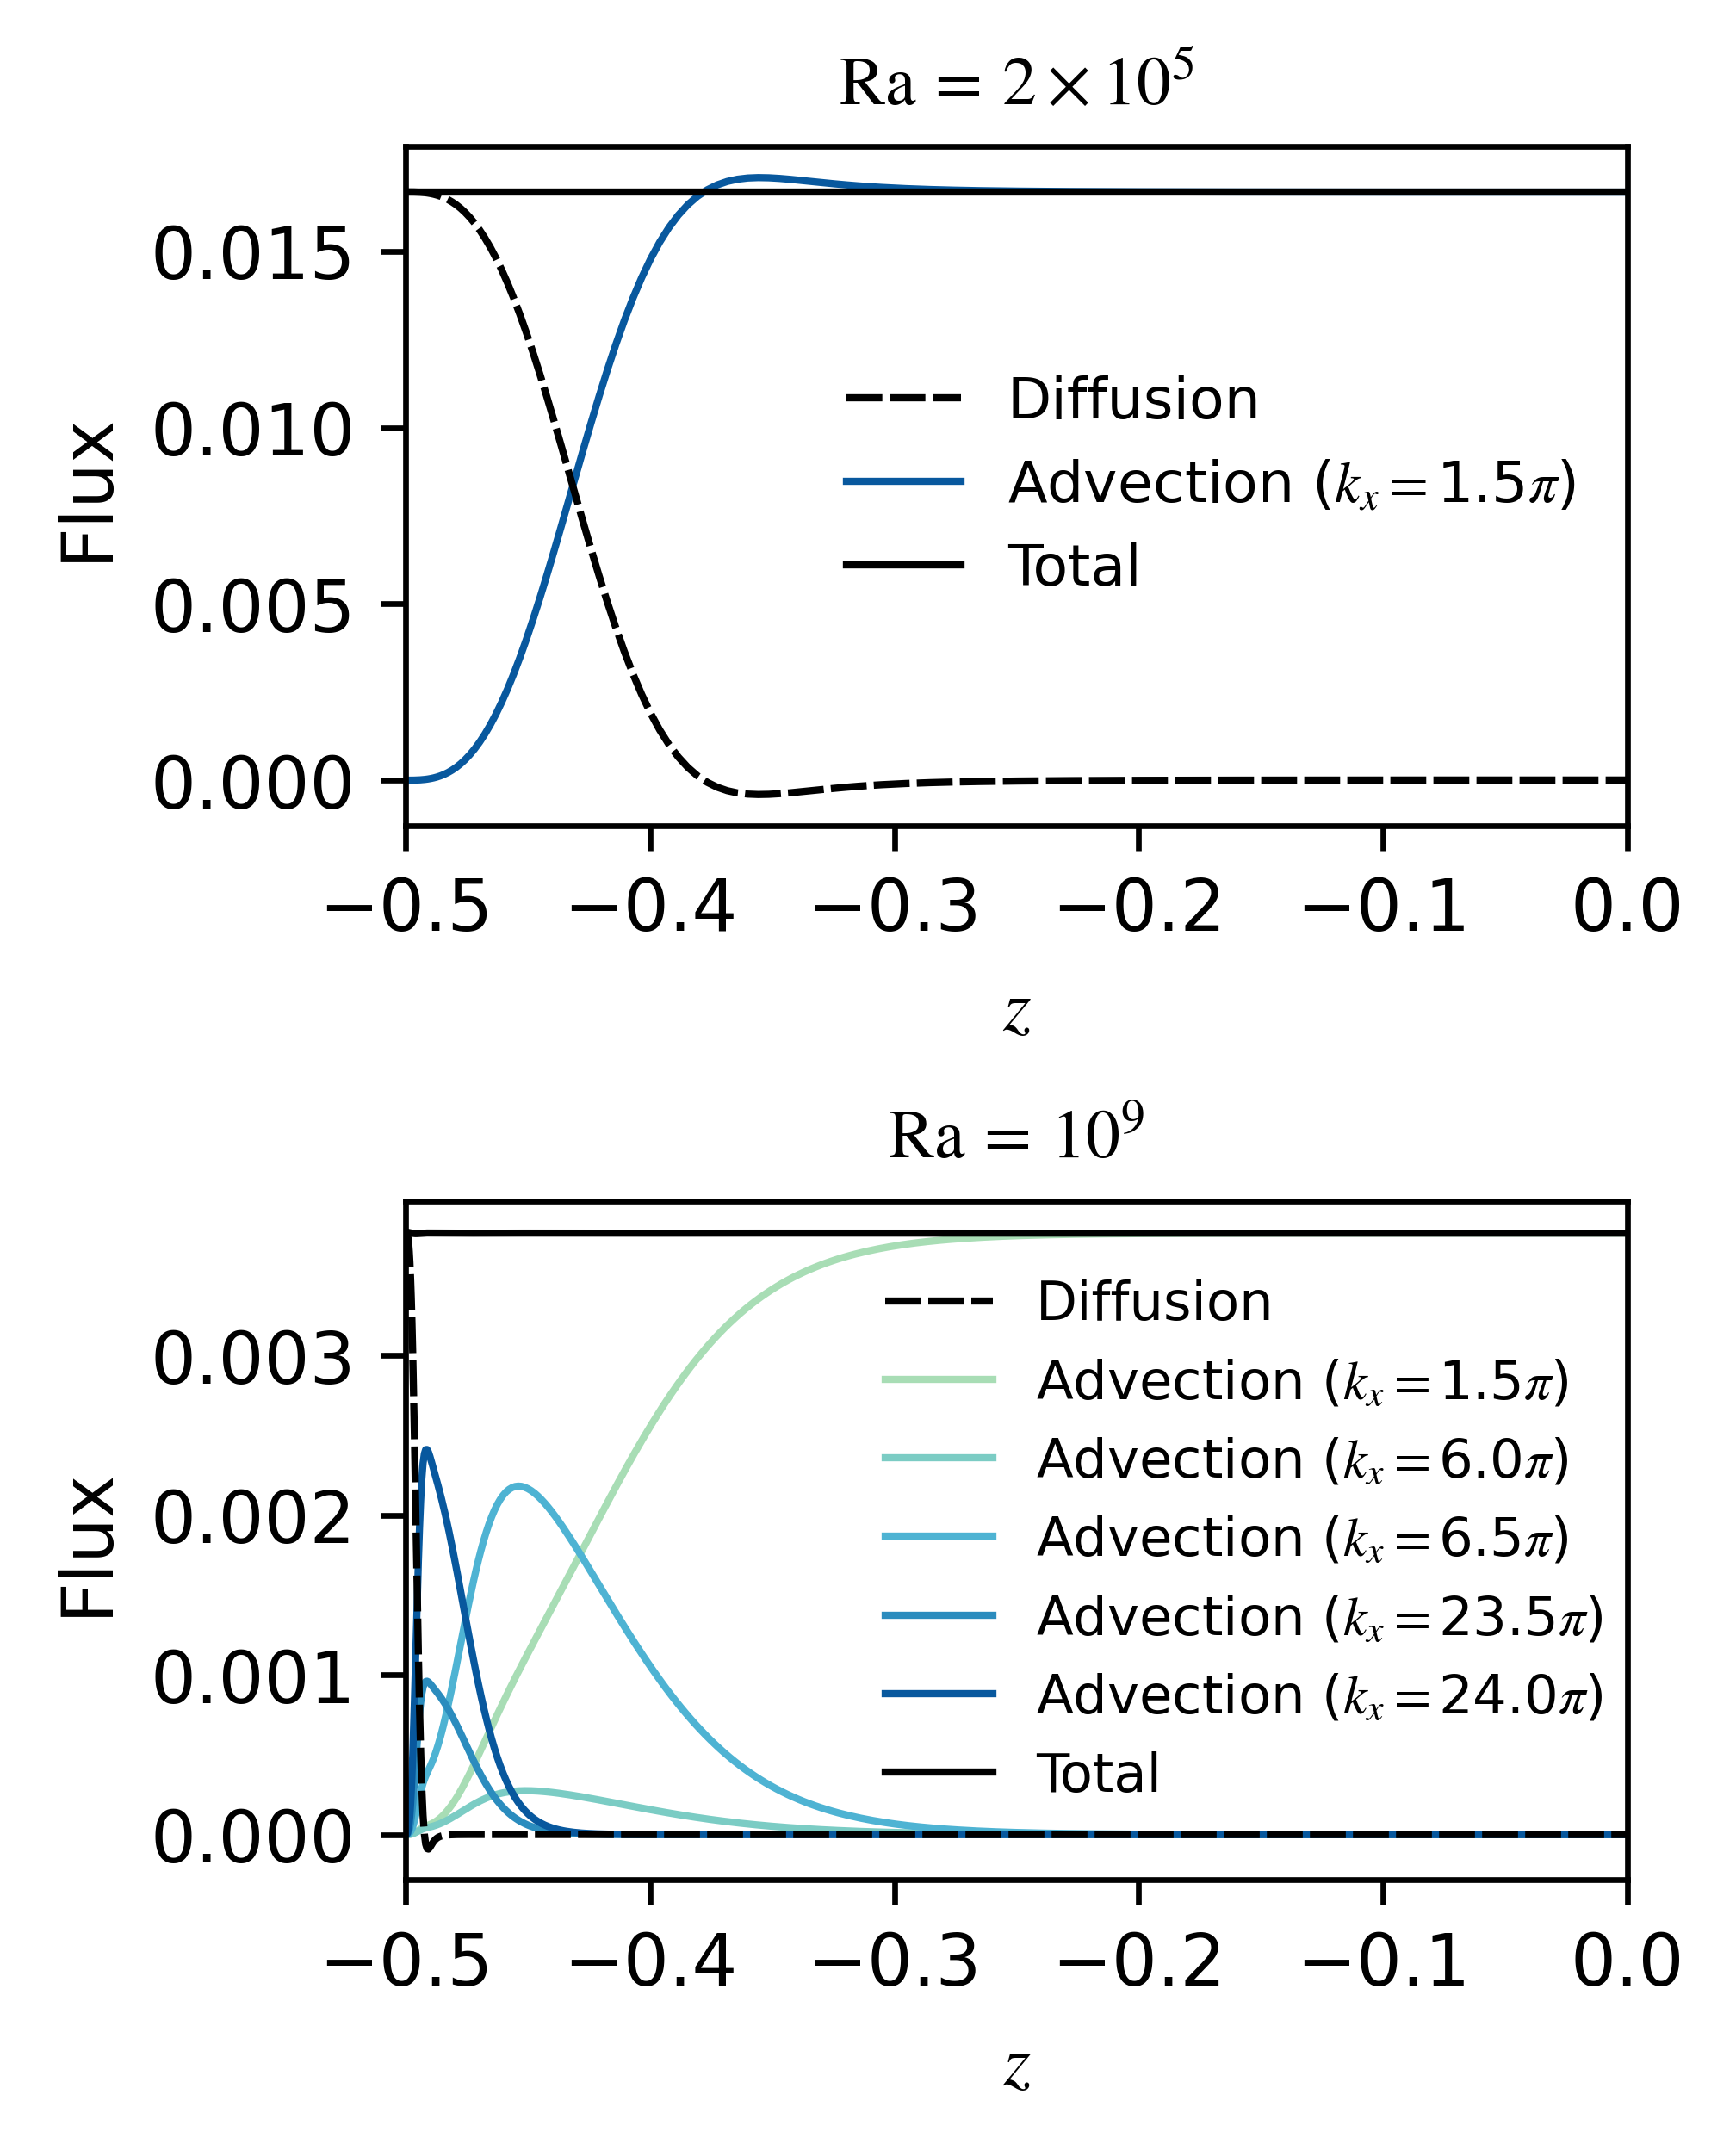
\includegraphics[width=3.4in]{flux_sup_n.png}
    \end{tabular}
    \begin{tabular}{@{}c@{}}
        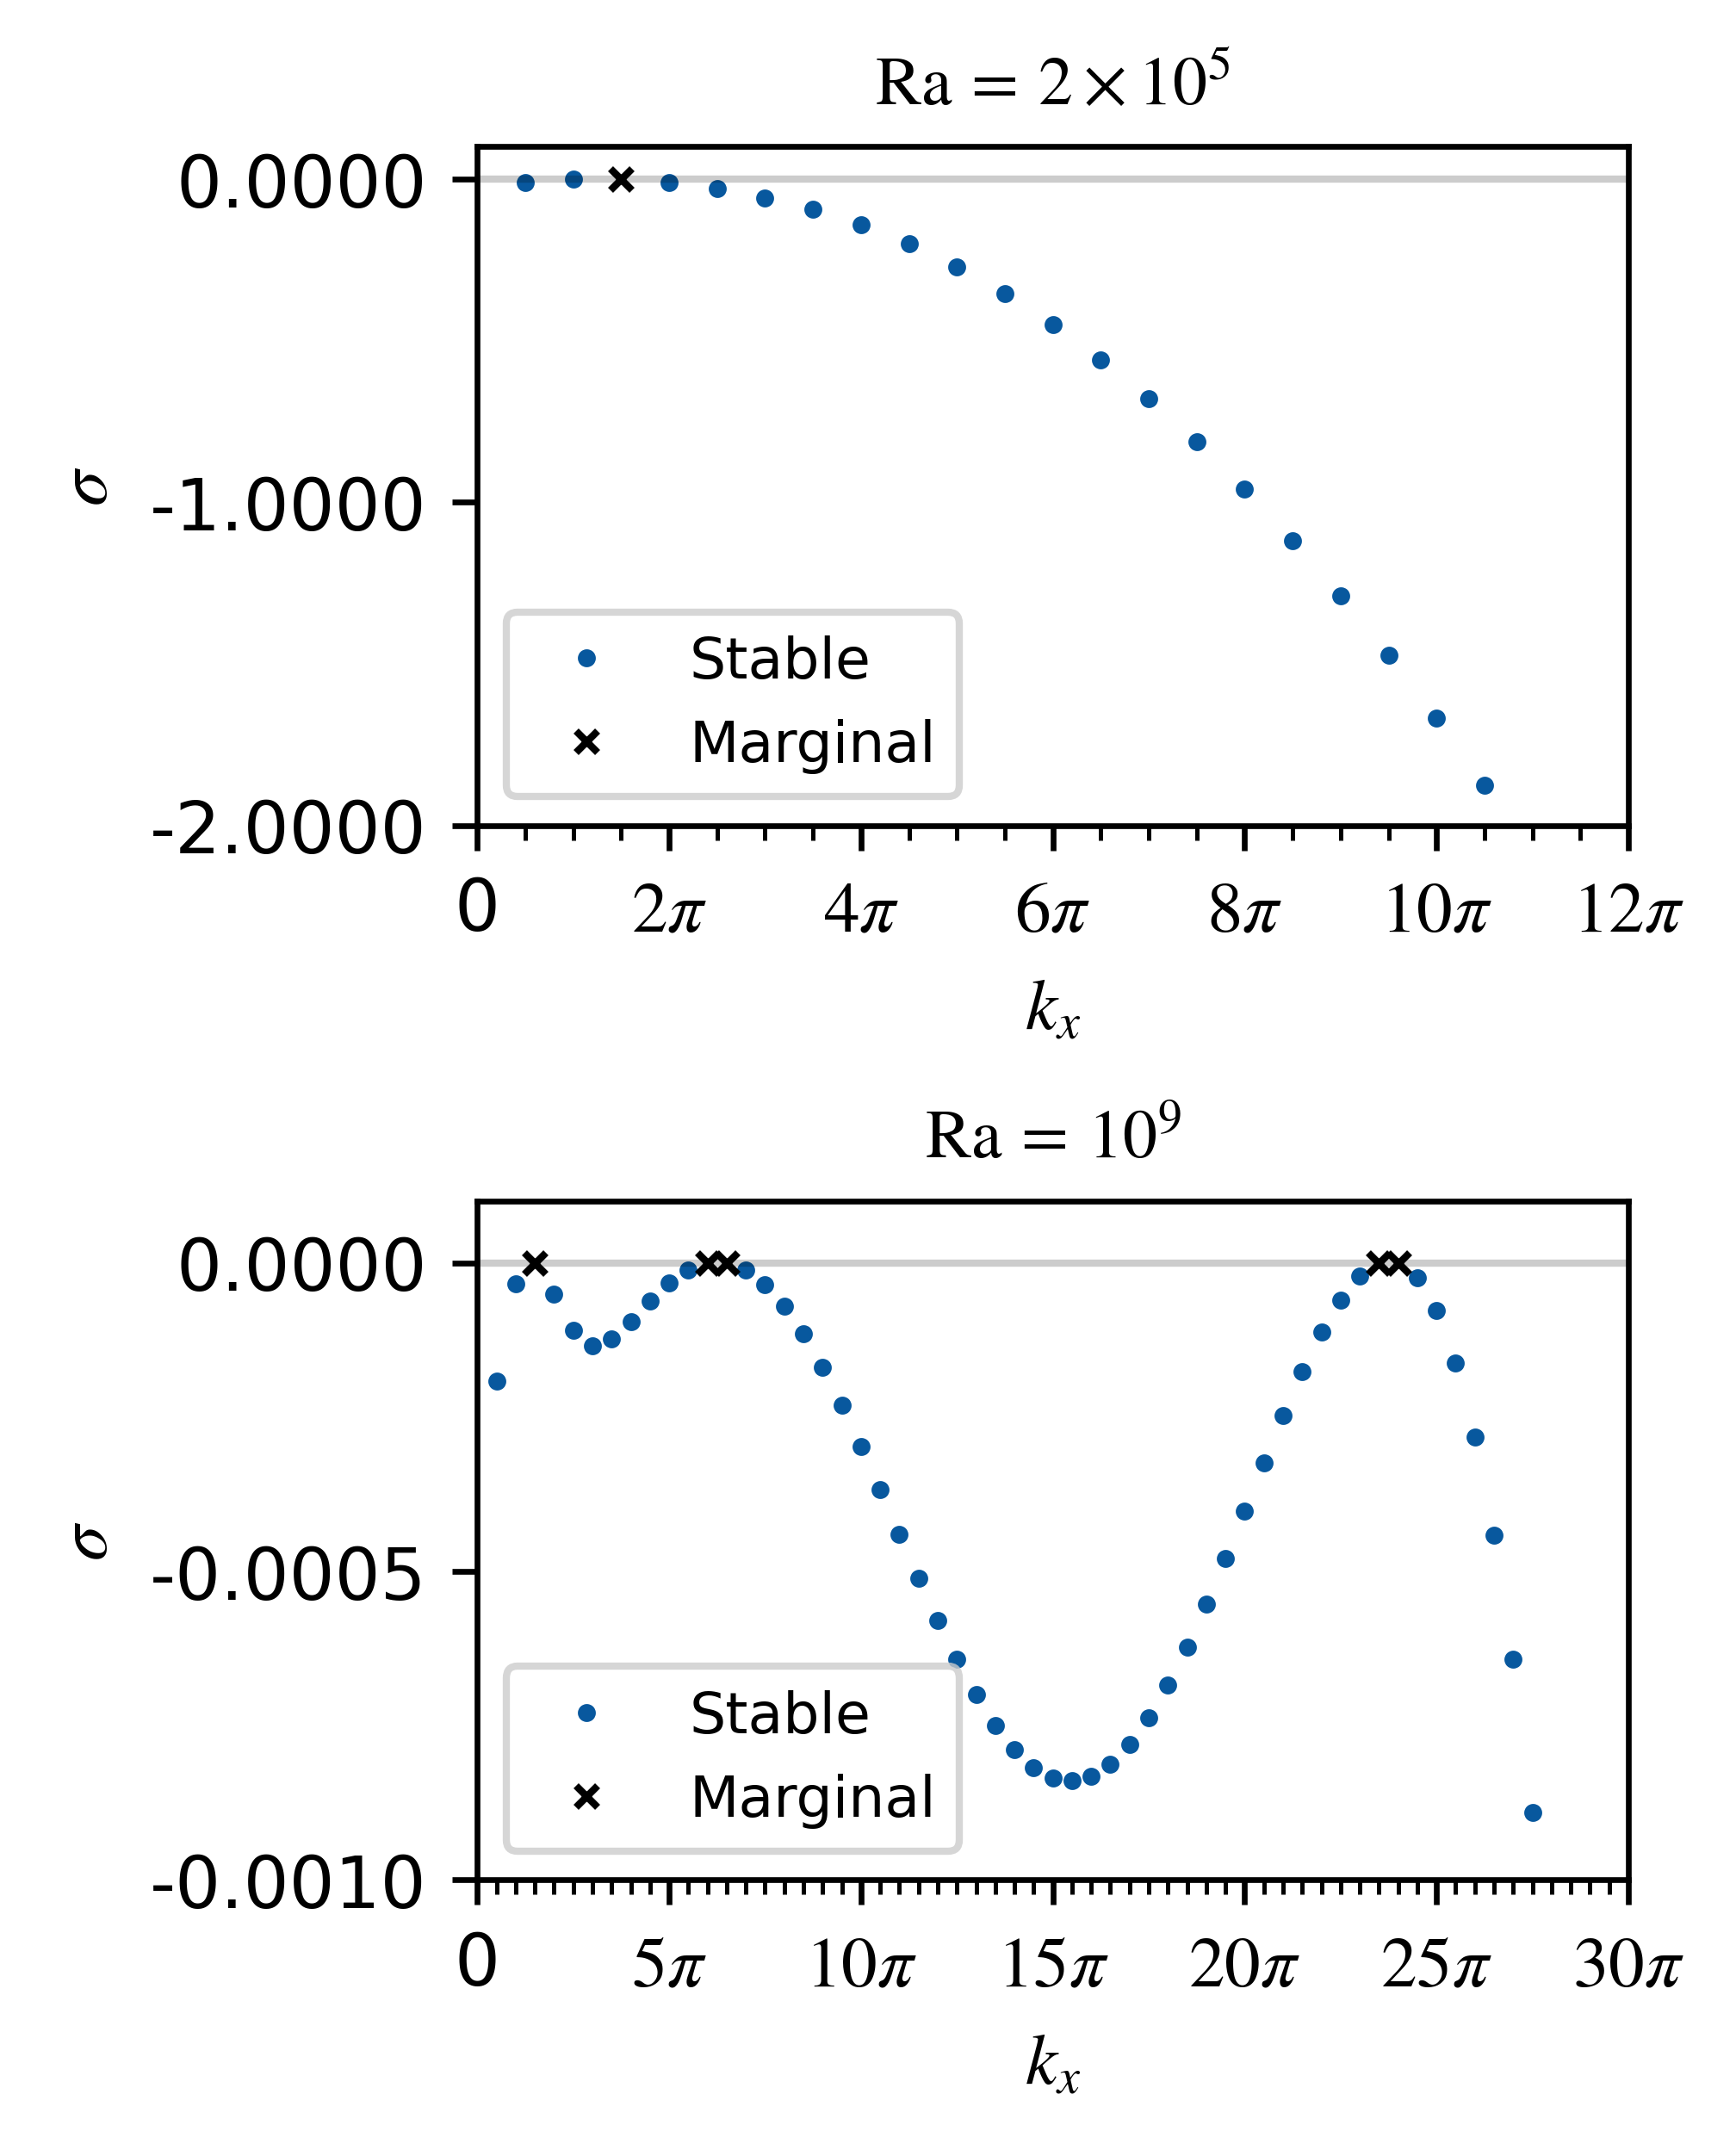
\includegraphics[width=3.4in]{EV_spectra_2ra.png}
    \end{tabular}
    \caption{Heat fluxes (left) and eigenvalue spectra (right) of equilibrated states $Ra = 2 \times 10^5$ (top) and $Ra = 10^9$ (bottom). 
    Advection profiles belong to marginally-stable modes. 
    For low $Ra$, a single mode with $k_x = 1.5\pi$ is sufficient to oppose boundary layer diffusion and facilitate heat flux throughout the bulk of the domain. 
    For large $Ra$, high-wavenumber modes contribute pronounced small-scale advection profiles which tightly hug the thin boundary layers. 
    A combination of of progressively wider advection profiles is necessary to transition to the $k_x = 1.5\pi$ mode.}
    \label{fig:flux}
\end{figure*}
\begin{figure*}
    \centering
    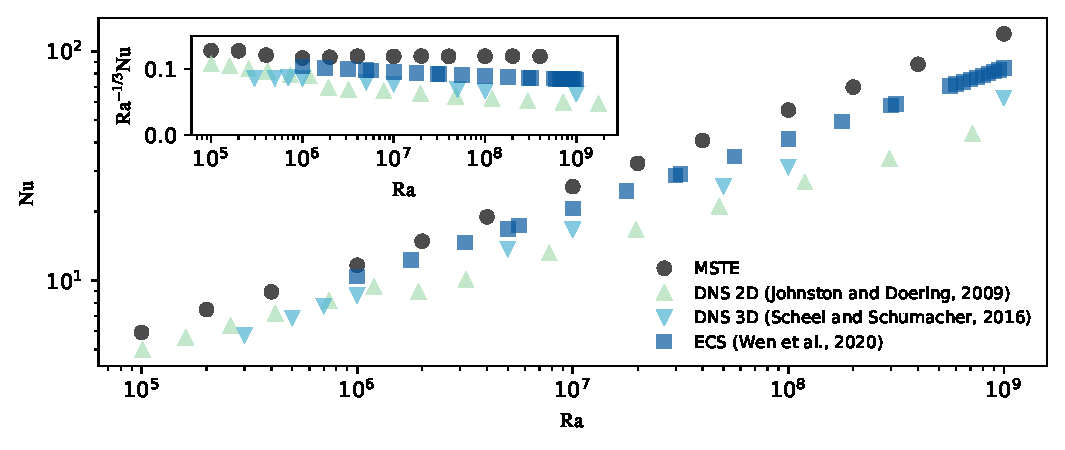
\includegraphics[width=7.1in]{nu_ra.PNG}
    \caption{Nusselt numbers are shown for marginally-stable thermally-equilibrated states, statistically-steady direct numerical simulations performed with \texttt{Dedalus} \cite{Anders_cd}, and equilibrated nonlinear solutions, which maximize heat flux, given by \cite{Waleffe}. 
    Both obey power-law relationships with $Ra$, with $Ra \sim \Nu^3$ in agreement with Figures \ref{fig:bl_ra}, \ref{fig:kx_marginals}, and \ref{fig:del_inv} as well as \cite{Malkus}. 
    Marginally-stable states' Nusselt numbers exceed simulation Nusselt numbers. 
    This can be well explained by the contrasting boundary region geometries shown in Figure \ref{fig:T0_profiles}.}%
    \label{fig:nu_vs_ra}%
\end{figure*}

\begin{figure}
    \centering
    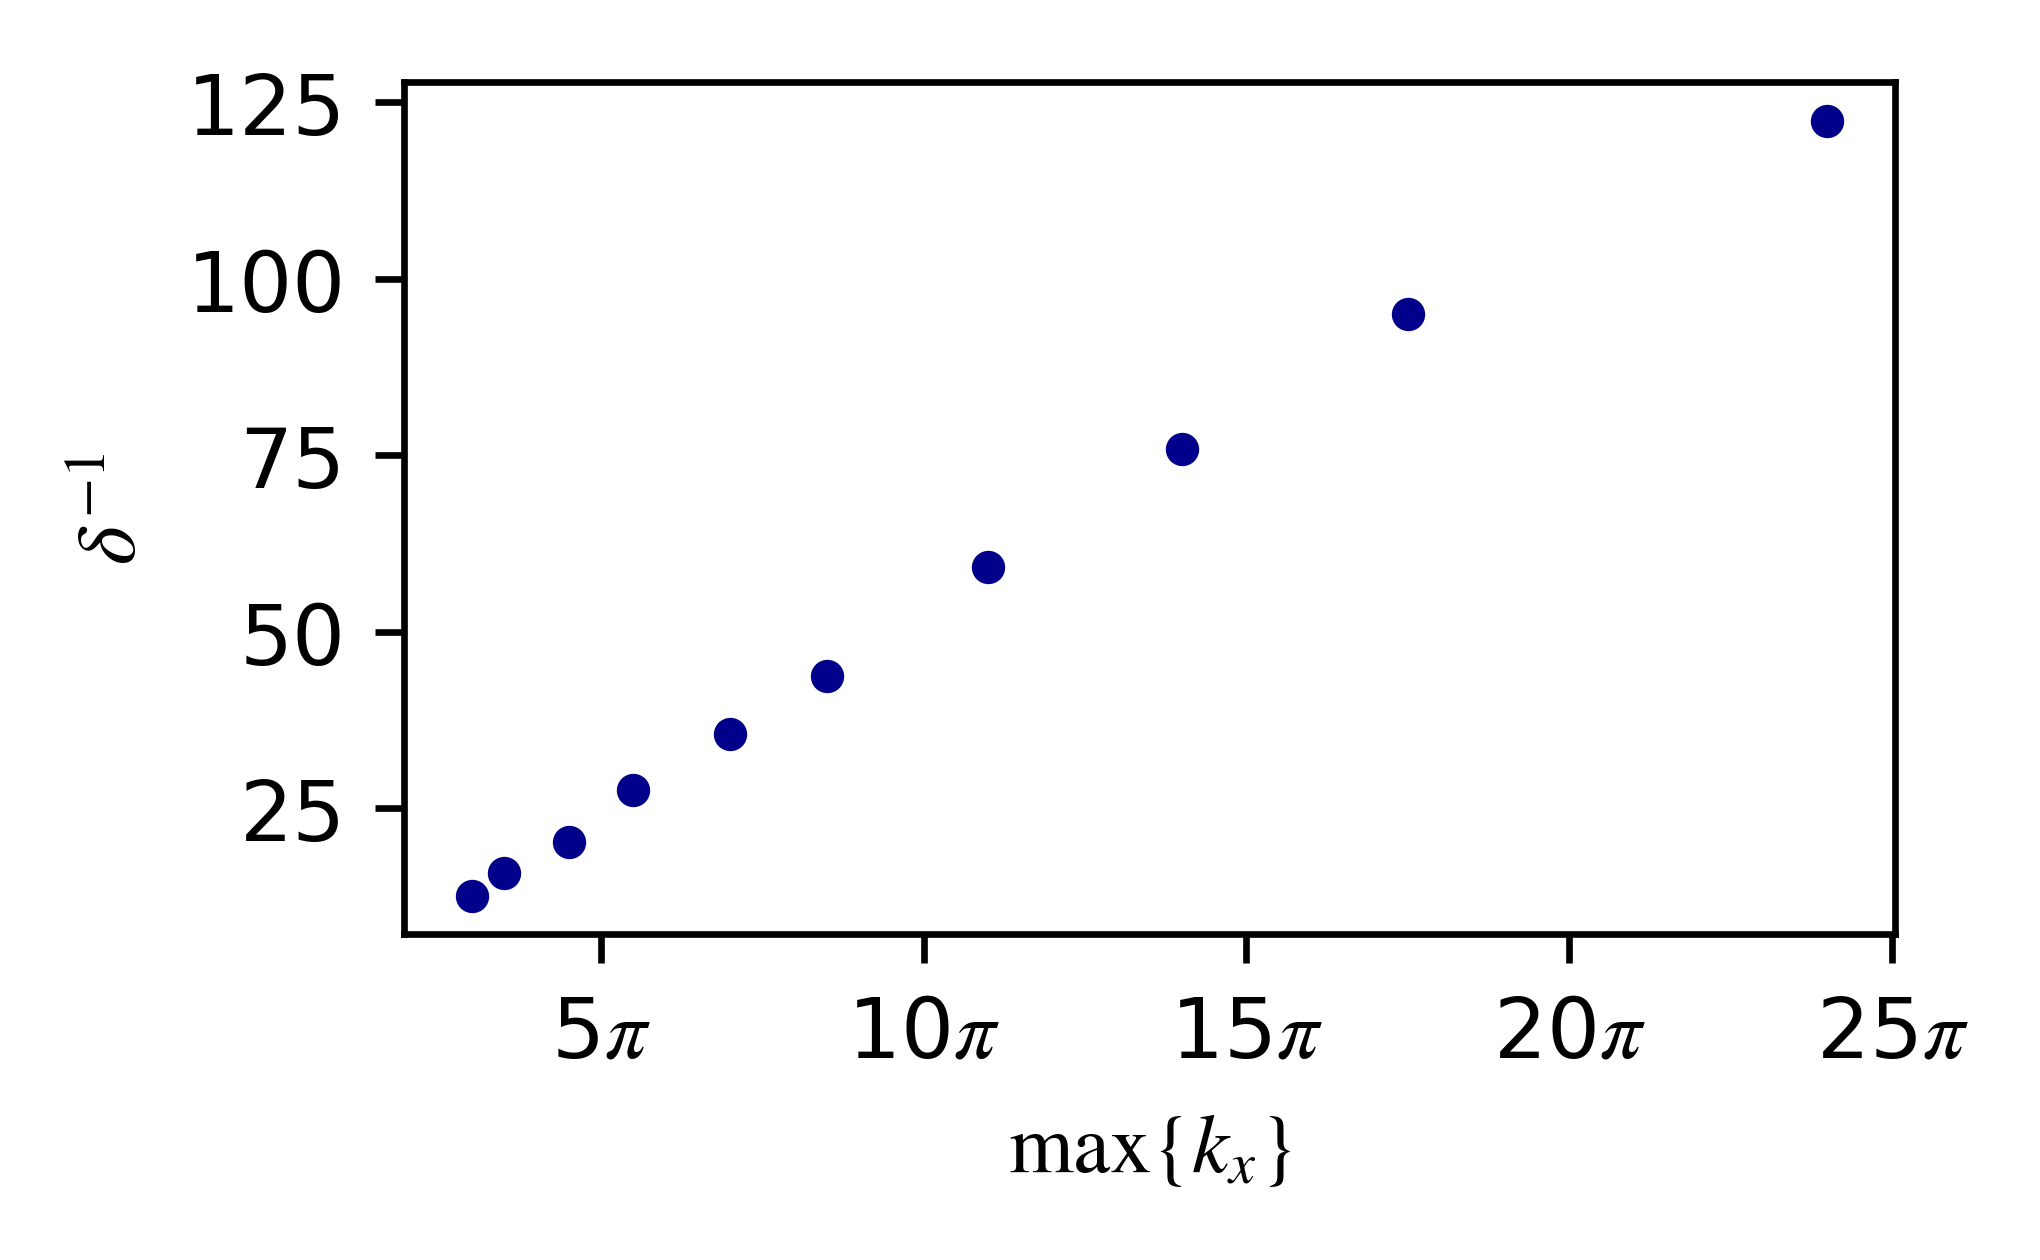
\includegraphics[width=3.4in]{del_kx_inv.png}
    \caption{For $Ra \geq 10^6$, the maximum marginally-stable wavenumber (corresponding to the green X markers in Figure \ref{fig:kx_marginals}) are inversely related to the boundary layer thicknesses $\delta$. 
    $(\max \{ k_x \})^{-1}$ gives a minimum $x$ length scale for the perturbations, and consequently, the advection. 
    We expect the minimum $z$ length scale to agree with the boundary layer thickness $\delta$ because otherwise the boundary layer would continue to diffuse. 
    This is illustrated in the lower left corner of Figure \ref{fig:flux}, where the advection profile for $k_x = 24\pi$ is tightly flanked by the surrounding boundary layers. 
    This suggests that the minimum $x$ and $z$ length scales obey some constant ratio.}
    \label{fig:del_inv}
\end{figure}

\begin{figure}
    \centering
    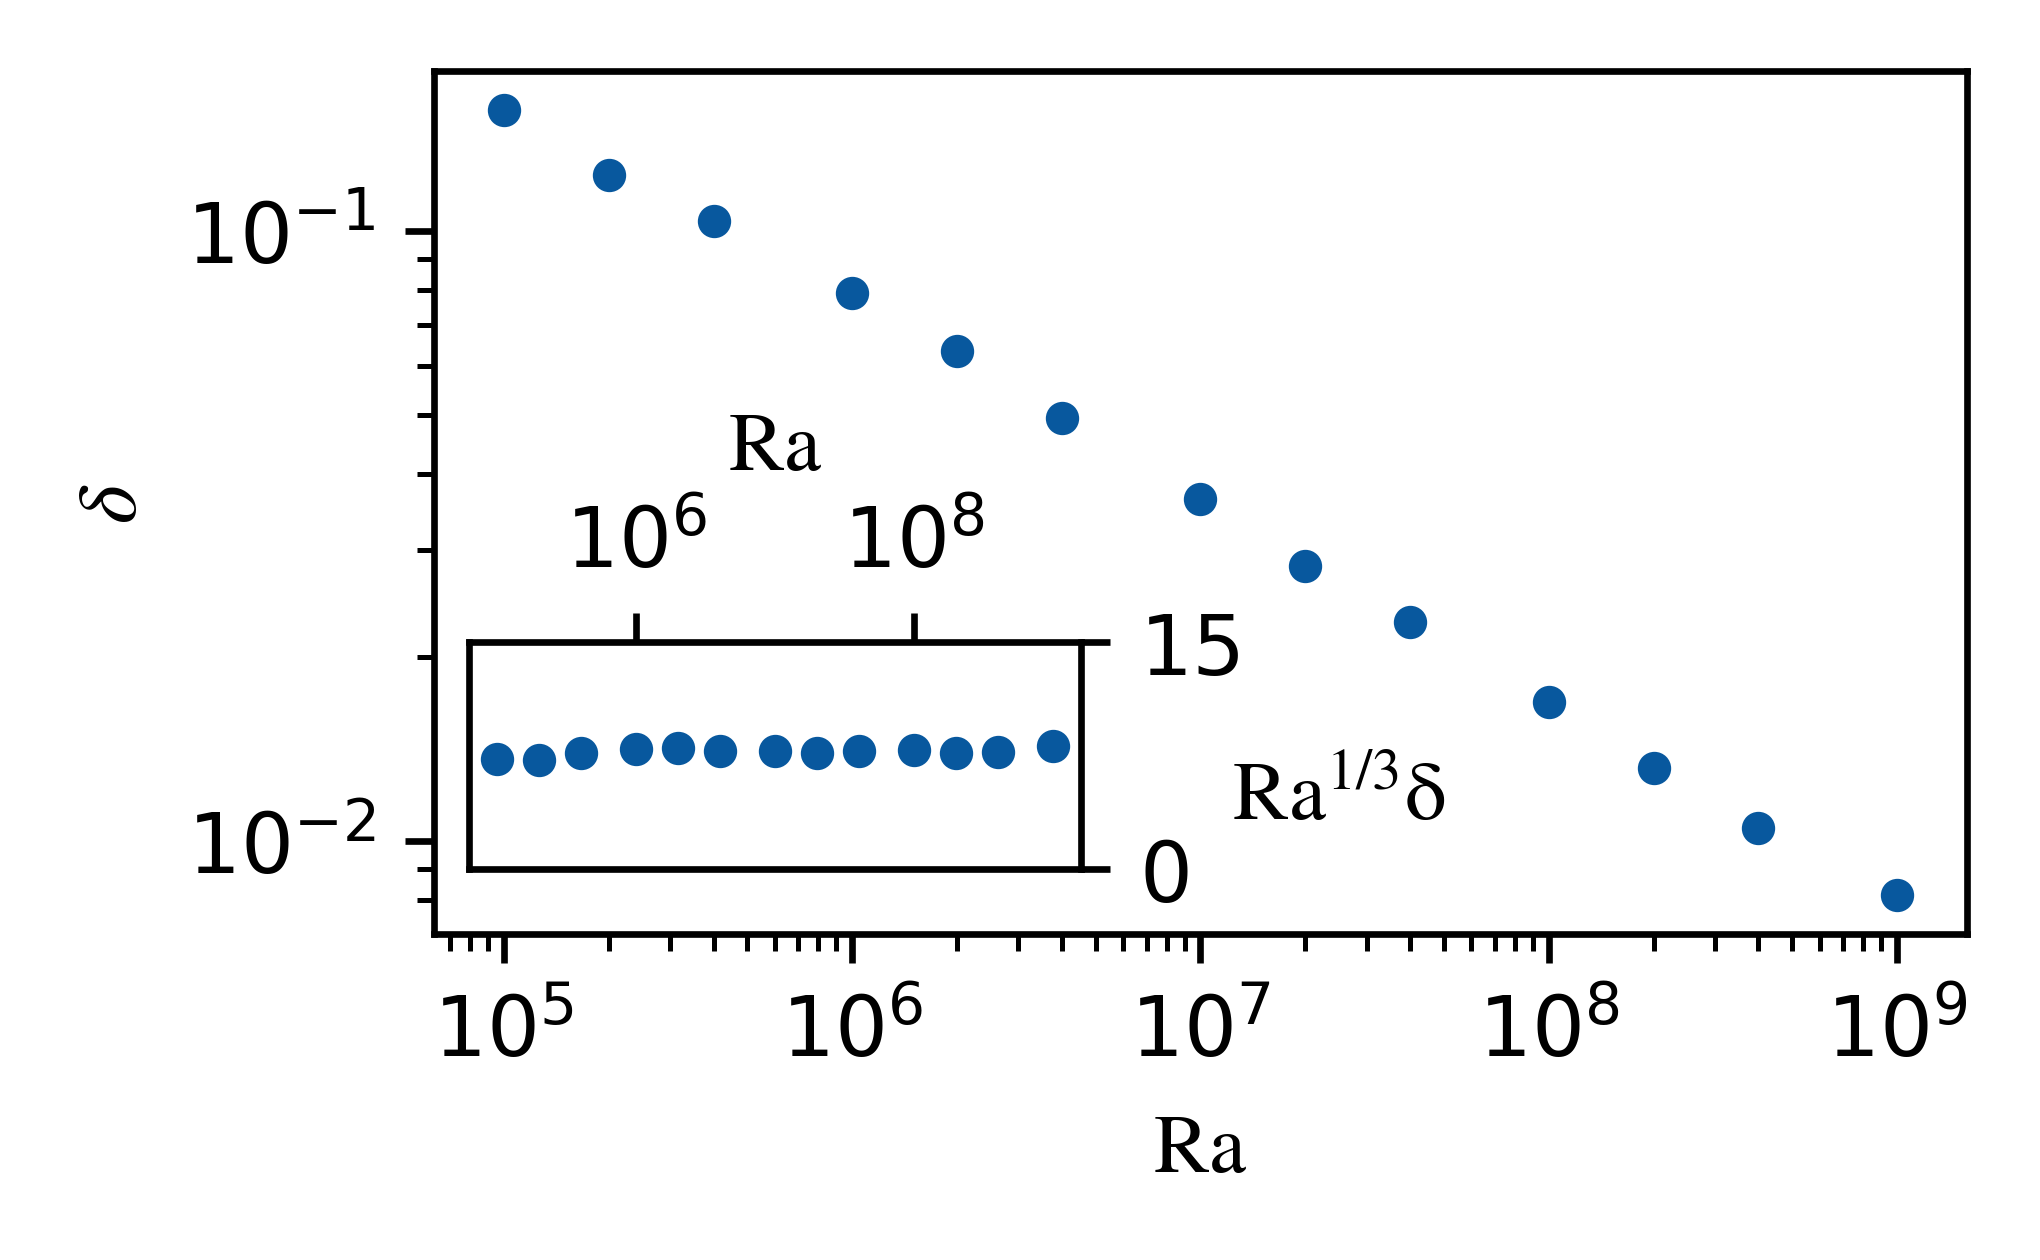
\includegraphics[width=3.4in]{del_ra.PNG}
    \caption{Boundary layer widths $\delta$ of marginally-stable thermal equilibria. 
    We define the threshold of each boundary layer as the $z$-coordinate at which $\frac{\partial \bar{T}}{\partial z} = 0$, corresponding to the local extrema of the equilibrated curve in Figure \ref{fig:T0_profiles}. 
    Plotting on a log-log scale, we find $\delta$ and $Ra$ obey a power-law relationship. We also demonstrate that $Ra^{1/3}\delta$ is approximately constant with respect to $Ra$ implying $Ra \propto  \delta^{-3}$, as predicted by \cite{Malkus}}
    \label{fig:bl_ra}
\end{figure}

Equilibrated states exhibit distinct behaviors for large and small $Ra$. 
This contrast is illustrated in Figure \ref{fig:flux}, where we give heat flux profiles and eigenvalue spectra for two cases: $Ra = 2 \times 10^5$ and $Ra = 10^9$. 
For lower $Ra$, there is a single presumed local maximum in the eigenvalue spectrum, whose adjacent modes' advection profiles occupy the bulk of the domain. 
These states have relaxed boundary layers which gradually subside as advection becomes the dominant component of the total flux. 
Such transitional regions do not appear in high $Ra$ cases, where the shift from diffusion to advection is sharp, requiring pronounced, small-scale advection profiles belonging to modes adjacent to the third presumed local maximum in the eigenvalue spectrum. 
Traversing towards the midplane of the domain, we see increasingly thicker advection profiles corresponding the wavenumbers adjacent to the second local maximum, eventually culminating in the dominant $k_x = 1.5\pi$ mode.

Thermally equilibrated states with large $Ra$ tend to have a more diverse set of marginal modes as compared to small $Ra$ states. 
In every case, the $k_x = 1.5\pi$ mode is included and is often unaccompanied by adjacent modes. 
In Figure \ref{fig:kx_marginals} we give the wavenumbers $k_x$ of marginal modes, color coded accordingly to their respective adjacencies. 
Marginal modes often appear in neighboring pairs, in which case the larger mode is denoted with an x and the smaller mode is denoted with a +. 
In these cases we infer the existence of a local maximum eigenvalue between the two adjacent marginally-stable modes. 
For $Ra \geq 10^6$, a second branch of marginal modes is introduced as shown in green, increasing according to some power-law with respect to $Ra$. 
The introduction of this largest branch is likely required to oppose the diffusion of the thinning boundary layers. 
For $Ra \geq 10^8$, a third branch appears (shown in red), splitting the widening gap between the blue branch and the green branch. 
This development is associated with relatively thick advection profiles, filling a niche in the total flux by uniting the sharp profiles of the largest branch (green) and those of the bulk-domain-oriented smallest branch (blue).

In general, marginally-stable thermal equilibria can be characterized by their boundary layer thicknesses, from which, the rest of their properties follow. Letting the interior boundary layer threshold be the $z$-coordinate at which $\frac{\partial \bar{T}}{\partial z} = 0$, we find that $Ra \propto  \delta^{-3}$ as illustrated in Figure \ref{fig:bl_ra}. 
This is consistent with Malkus' classical marginal-stability theory, a scaling argument which perceives the boundary regions as subdomains which are themselves marginally-stable.

Nusselt numbers $\Nu$ of various solutions are given in Figure \ref{fig:nu_vs_ra}. 
The marginally-stable thermally-equilibrated states and numerical simulation data exhibit power-law relationships with $Ra$. 
More specifically, $Ra \sim \Nu^3$ which agrees with Figures \ref{fig:bl_ra}, \ref{fig:kx_marginals}, and \ref{fig:del_inv} and the scaling argument given by \cite{Malkus}. 
The nonlinear solutions, which maximize heat flux, are obtained by \cite{Waleffe}. 
$\Nu$ of both equilibria exceed that of simulations, which might be due to the transitional behaviors outlined by \cite{Yalniz} and \cite{Cvitanovic} inhibiting heat flux. 
Alternatively, we might anticipate the existence of exact coherent states with smaller $\Nu$, forming another node in the Markov chain whose long-term behavior agrees with the simulation data.

\section{Simulations with Thermally Equilibrated Initial Conditions}
This investigation is partially motivated by the prospect of decreasing nonlinear simulation relaxation times by employing thermally-equilibrated initial conditions. 
Conventionally, (\ref{EQ:motion1}) - (\ref{EQ:motion3}) are solved via direct numerical simulation (DNS) with initial conditions
\begin{align}
    T(x, z)\big|_{t=0} &= 0.5 - z \\
    \mathbf{u}(x, z)\big|_{t=0} &= \mathbf{0} \\
    p(x, z)\big|_{t=0} &= 0
\end{align}
which will hereby be referred to as the conductive initial condition. 
$t$ in this section now refers to the simulation time as opposed to the thermal equilibration time parameter used previously. 
We define the equilibrated initial conditions
\begin{align}
    T(x, z)\big|_{t=0} &= \bar{T}(z) + \sqrt{2} \sum_{n=1}^N  A_n \text{ Re} \Big[ \theta_n(z) e^{ik_{x_n}x} \Big] \nonumber \\
    \mathbf{u}(x, z)\big|_{t=0} &= \sqrt{2} \sum_{n=1}^N A_n \text{ Re} \Big[\Big( U_n (z) \hat{x} + W_n(z) \hat{z} \Big) e^{ik_{x_n}x} \Big] \nonumber\\
    p(x, z)\big|_{t=0} &= \sqrt{2} \sum_{n=1}^N A_n \text{ Re} \Big[P_n (z) e^{ik_{x_n}x}\Big]
\end{align}
Where $\theta_n(z), U_n(z), W_n(z), P_n(z); \, A_n; $ and $k_{x_n}$ refer to the complex eigenfunctions, amplitude, and wavenumber at the $n$th marginal mode respectively. 
The $\sqrt{2}$ factor is necessary for eigenfunction normalization. 
By construction, these initial conditions are thermally equilibrated. 
Simulations launched with equilibrated initial conditions do not exhibit a convective-transient period, as the large-scale anatomy of plumes and convective winds which are characteristic of Rayleigh-B\'enard convection exist on initialization. 
This is illustrated in Figure \ref{fig:nu_sim}, where the sharp spike in $\Nu$ is associated with a turbulent transitional period of upwelling until the distinctive jet-like structure is established. 
% \begin{figure}
%     \centering
%     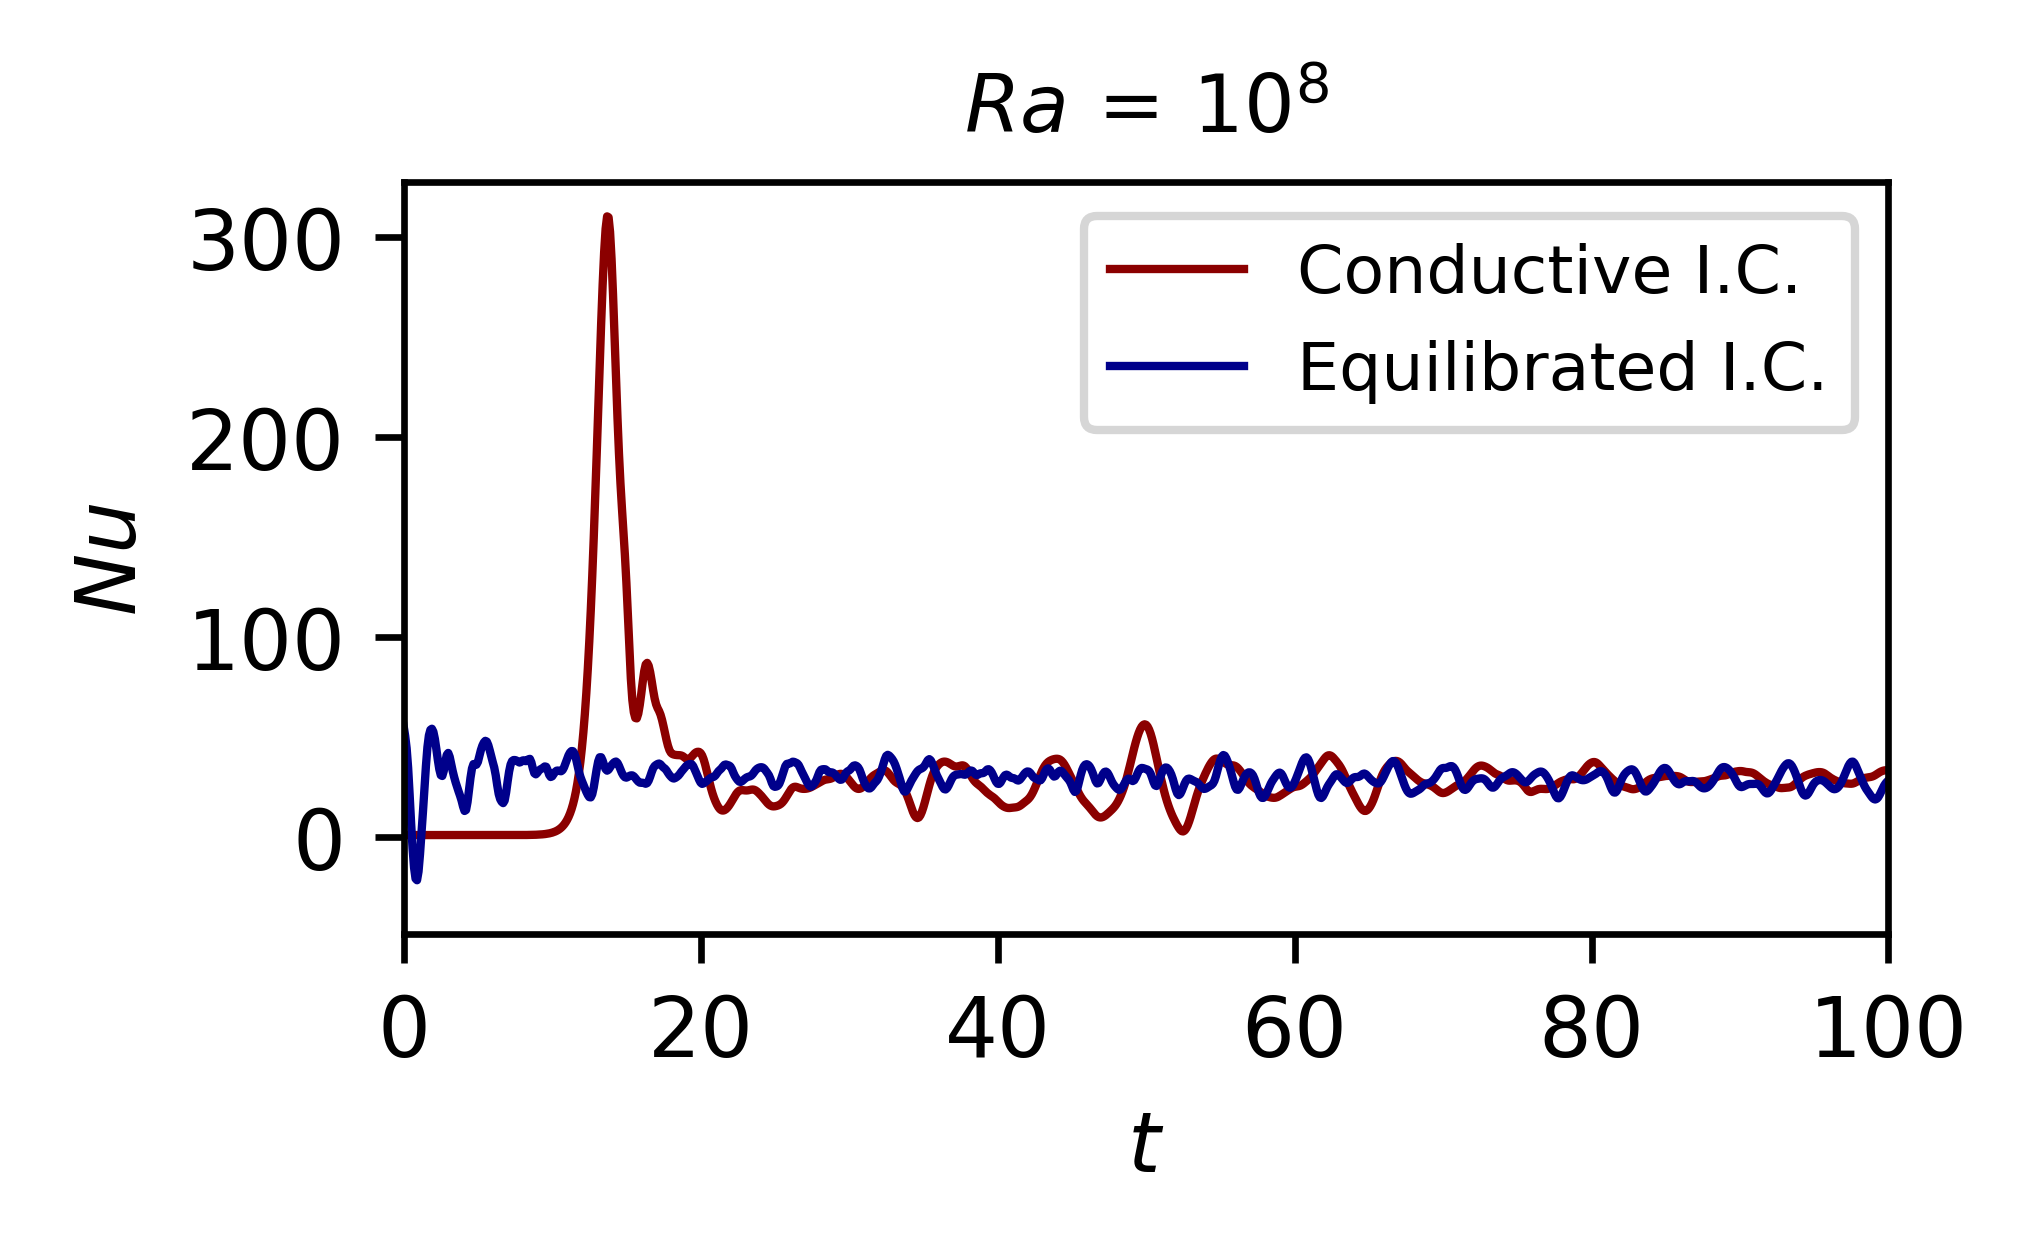
\includegraphics[width=3.4in]{sim_eq_nu.png}
%     \caption{Nusselt numbers of simulations performed at $Ra \, = \, 10^8$ with conventional initial conditions (red) and marginally-stable thermally-equilibrated initial conditions (blue). Simulations launched with thermally-equilibrated states do not undergo a convective-transient period because the characteristic plume structure exists on initialization. This is illustrated by the $Nu$ spike at $t \sim 15$ in the convectional simulation.}
%     \label{fig:nu_sim}
% \end{figure}
The marginally-stable equilibria are associated with a combination of eigenfunctions whose average kinetic energy is significantly larger than the statistical steady state, as given by Figure \ref{fig:ke_sim}. 
This is postpones kinetic relaxation because the large horizontal flows decay on a viscous timescale
\begin{equation}
    t_{\nu} \sim \sqrt{\frac{Ra}{Pr}}. \nonumber
\end{equation}
Consequently, marginally-stable thermally-equilibrated initial conditions do not reduce the simulation time required to achieve a statistically steady state, rather, they increase it considerably.
% \begin{figure}
%     \centering
%     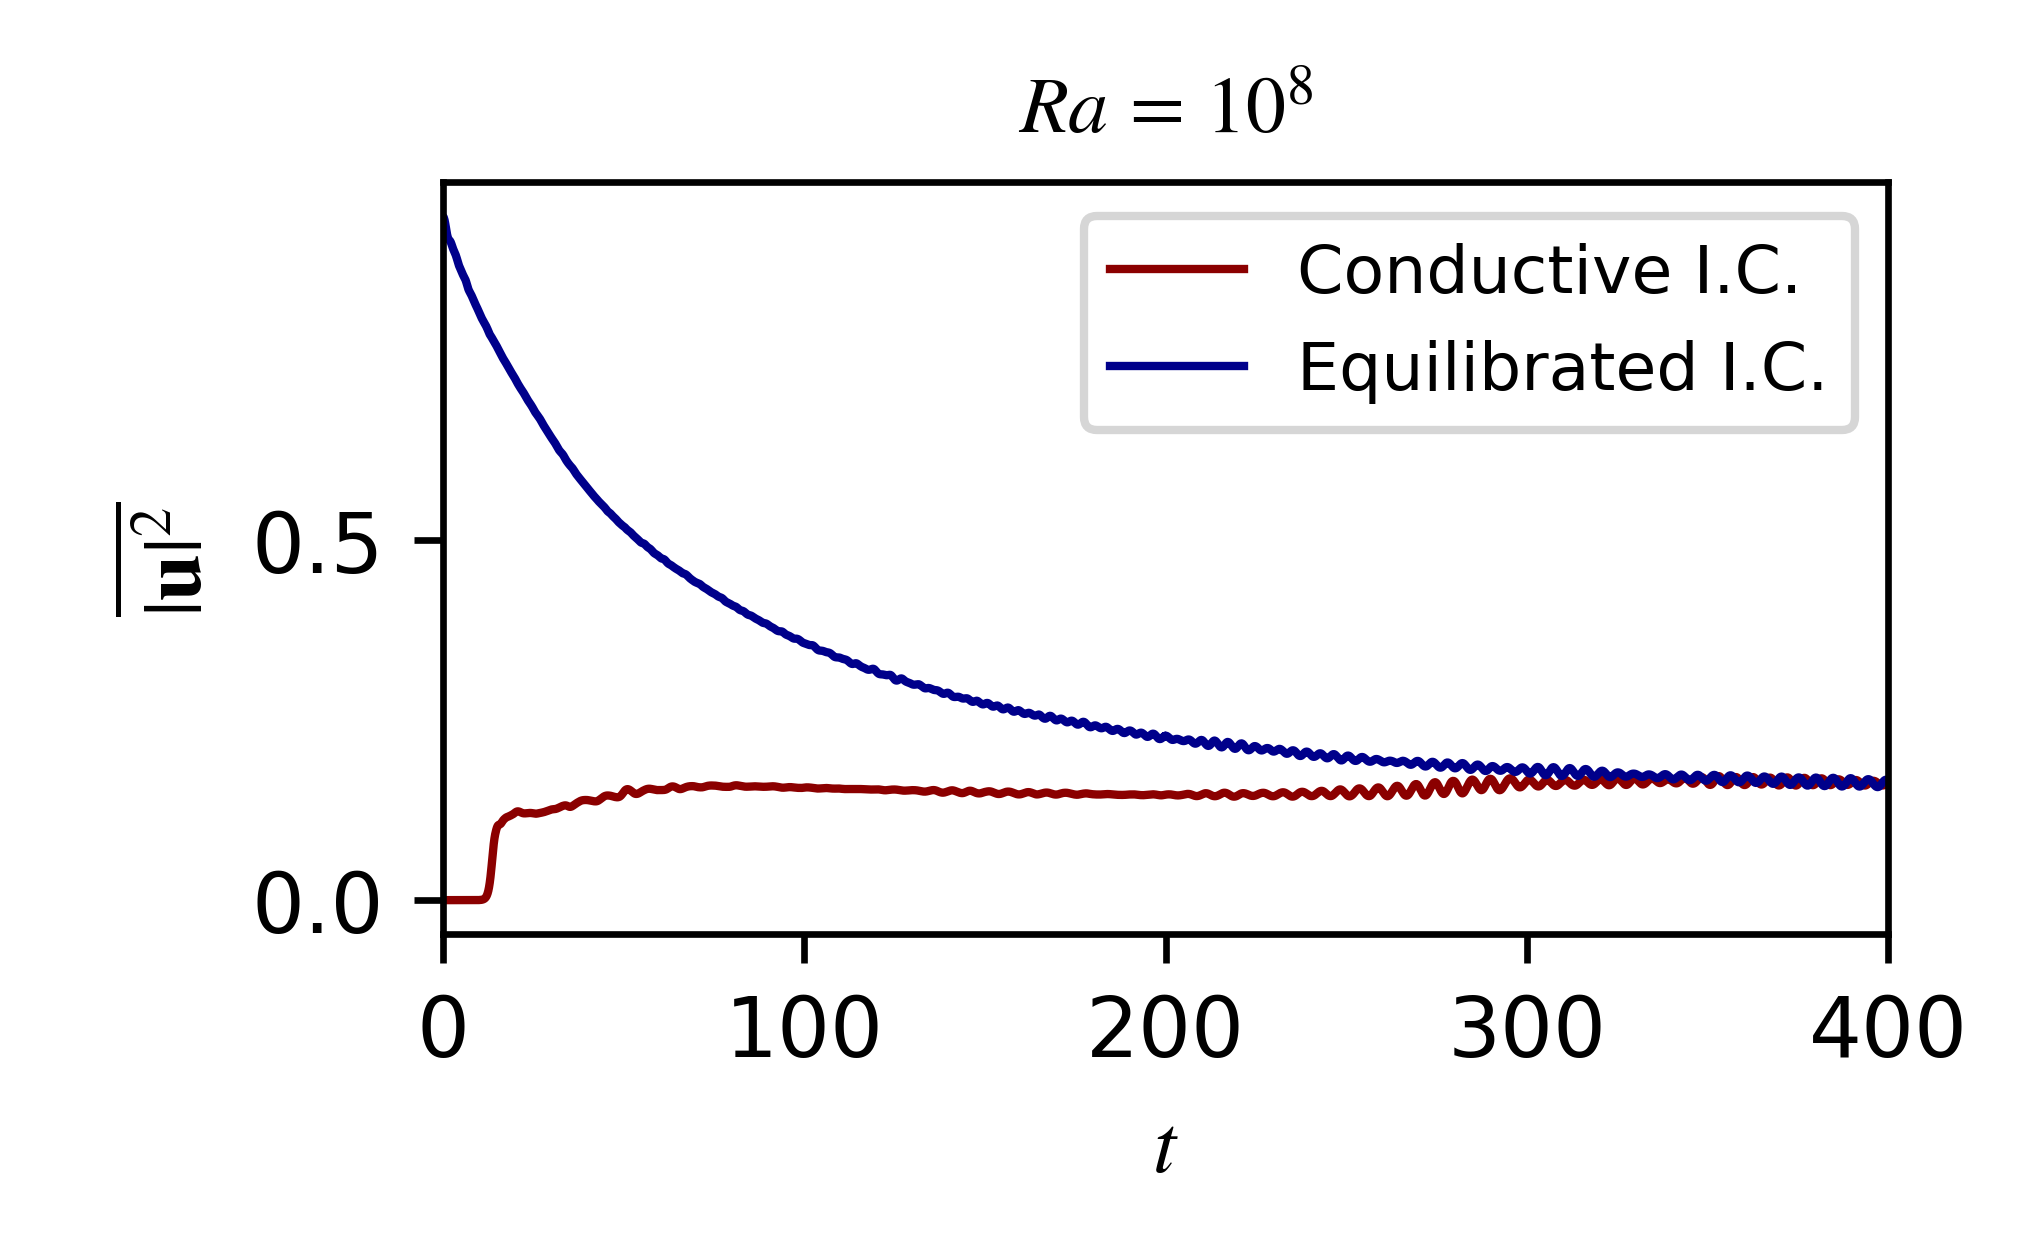
\includegraphics[width=3.4in]{sim_eq_ke.png}
%     \caption{Average kinetic energies of the same simulations performed in Figure \ref{fig:nu_sim} ($Ra = 10^8$). The combination of eigenfunctions which give thermal equilibrium have significantly more kinetic energy than the statistically steady state. Kinetic equilibrium is achieved according to the viscous timescale $t_{\nu} \sim Pr Ra^{-1/2}$.}
%     \label{fig:ke_sim}
% \end{figure}
\begin{figure}
    \begin{minipage}{3.4in}
        \centering
        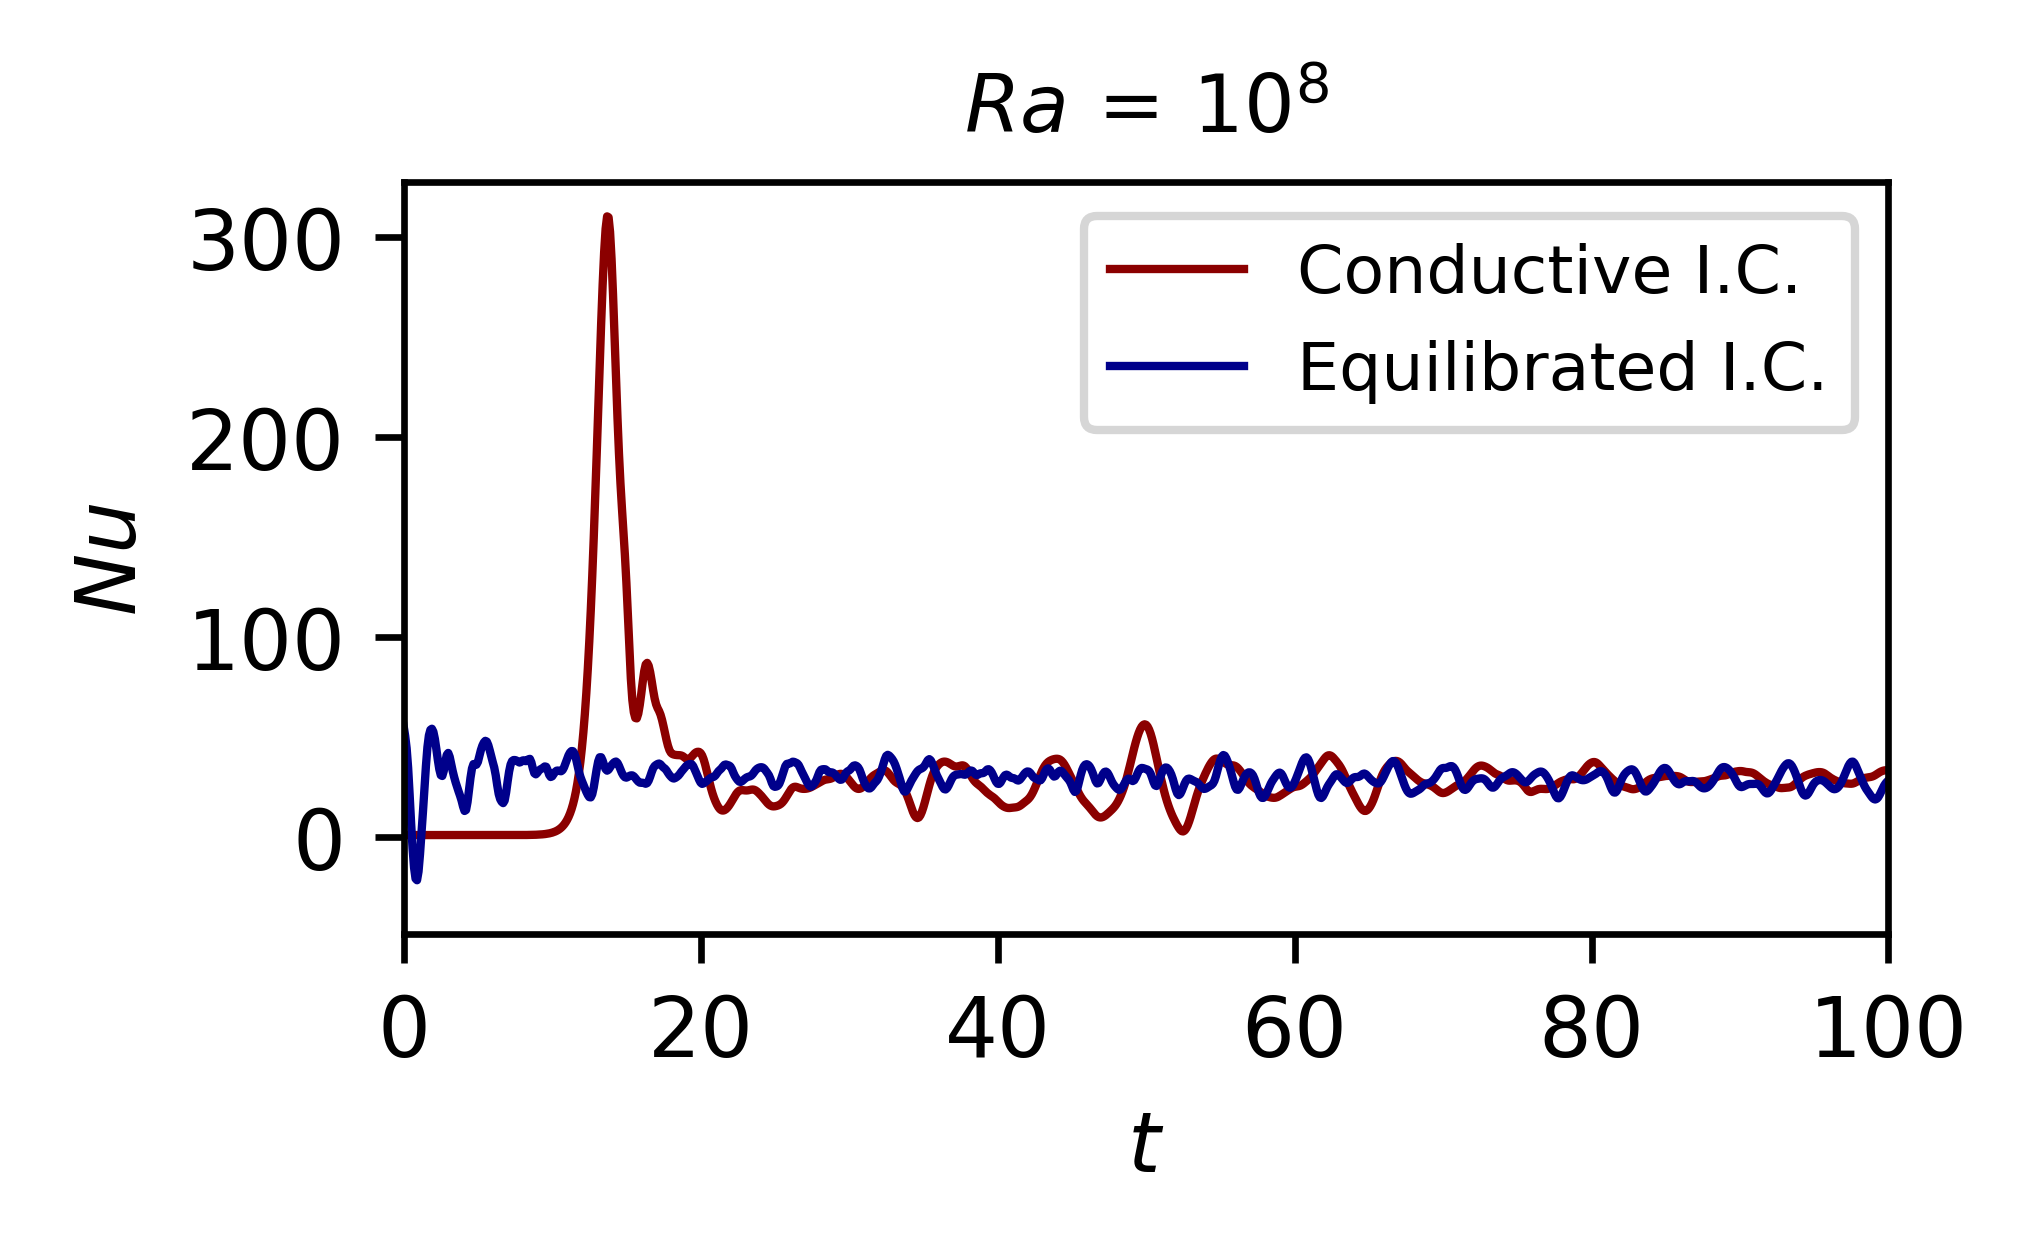
\includegraphics[width=3.4in]{sim_eq_nu.png}
        \caption{Nusselt numbers of simulations performed at $Ra \, = \, 10^8$ with conventional initial conditions (red) and marginally-stable thermally-equilibrated initial conditions (blue). 
        Simulations run with thermally-equilibrated states do not undergo a convective-transient period because the characteristic plume structure exists on initialization. 
        This is illustrated by the $\Nu$ spike at $t \sim 15$ in the convectional simulation.}
        \label{fig:nu_sim}
    \end{minipage}
\end{figure}

\begin{figure}
    \begin{minipage}{3.4in}
        \centering
        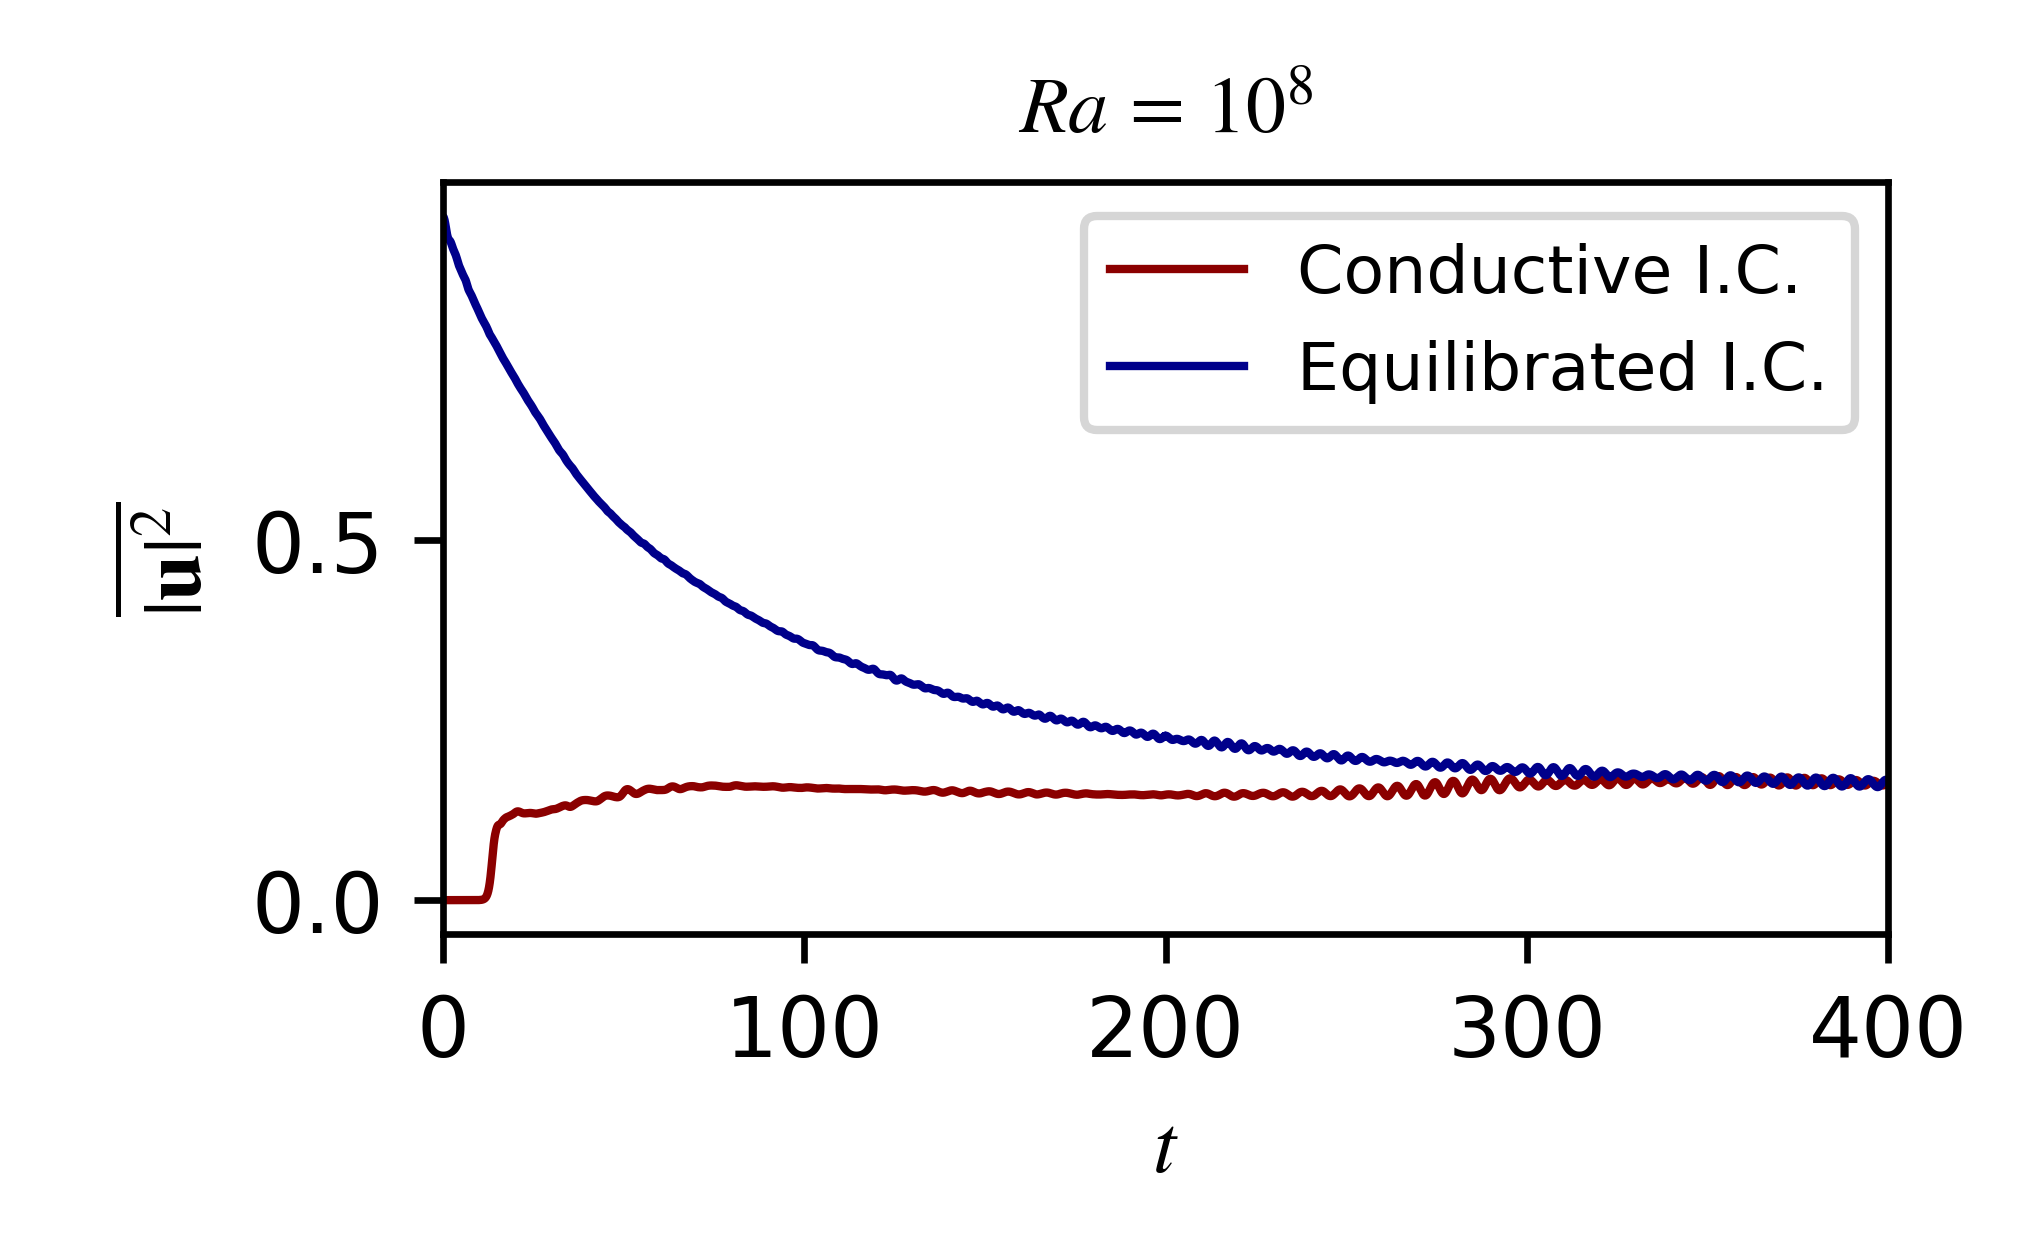
\includegraphics[width=3.4in]{sim_eq_ke.png}
        \caption{Average kinetic energies of the same simulations performed in Figure \ref{fig:nu_sim} ($Ra = 10^8$). 
        The combination of eigenfunctions which give thermal equilibrium have significantly more kinetic energy than the statistically steady state. 
        Kinetic equilibrium is achieved according to the viscous timescale $t_{\nu} \sim \sqrt{Ra / Pr}$.}
        \label{fig:ke_sim}
    \end{minipage}
\end{figure}

\section{Discussion}\label{sec:Discussion}
In general, the reduced model we study in this paper can be perceived as a unique way to describe Rayleigh–Bénard convection. 
Solutions to the quasilinear problem retain several key features that are ubiquitous in experiments and simulations: power-law $\Nu$ scaling, plume-like structures, and minimum length-scale approximations \cite{Malkus}. 
They also exhibit unique and unexpected features: gradient-reversal/dips in temperature profiles, kinetic exaggeration, and greater $\Nu$ than other time-invariant solutions. 
We also obtain indistinguishable solutions despite initializing with different mean temperature profiles $\bar{T}$. 
Thus solutions might be unique, but we cannot demonstrate this rigorously.

The quasilinear problem can also be generalized to include an asymmetric mean horizontal-flow. 
Specifically, a second initial value problem, similar to (\ref{EQ:T0_IVP}), can be derived for $\bar{u}$. 
Doing so might yield solutions with greater resemblance to DNS results because we expect the Reynolds stress tensor to combat the kinetic exaggeration shown in Figure \ref{fig:ke_sim}. 
For this investigation, we require symmetry at each iteration, but the thermal evolution procedure appears unstable to asymmetry. 
This could be accommodated by requiring rotational symmetry about the midplane $\bar{u}(z, t) = -\bar{u}(-z, t)$. 
It's unclear whether solutions with nontrivial $\bar{u}$ exist or whether our algorithm would converge under these different circumstances.

\section*{Appendix}
\subsection{Initial buoyancy profile} \label{sec:initial_profile}
In an attempt to minimize the required number of iterations, we initialize with \cite{Shishkina}'s analytical thermal boundary layer equation for turbulent Rayleigh-B\'enard convection, given by 
\begin{align}
    \bar{T}_0(\xi) &= \frac{\sqrt{3}}{4\pi} \log \frac{(1 + a\xi)^3}{1 + (a\xi)^3} + \frac{3}{2\pi} \arctan \Big( \frac{4\pi}{9}\xi - \frac{1}{\sqrt{3}} \Big) + \frac{1}{4} \nonumber \\
    \xi &= \frac{z}{\delta_0}, \qquad a = \frac{2\pi}{3\sqrt{3}}\label{EQ:T0}
\end{align}
where $\delta_0$ is the boundary layer thickness. 
We expect that each $\Ra$ is associated with a unique $\delta_0$ for which $\bar{T}_0(z)$ is marginally-stable. 
It should be noted that when experimenting with various initial profiles $(\tanh, \rm{erf}, \rm{etc.})$, we obtain indistinguishable equilibrated states, implying that solutions may be unique. 
An example of (\ref{EQ:T0}) is given by the blue curve in Figure \ref{fig:T0_profiles}.

\section*{Acknowledgments}
The authors thank Jeff Vassil, Greg Chini, Emma Kaufman for their valuable feedback and suggestions. 
We also thank the \texttt{Dedalus} and \texttt{Eigentools} development teams. 
Computations were performed on the NASA Pleiades system.

% \bibliography{she}
\begin{thebibliography}{99} 

\bibitem{Zhu} Xiaojue Zhu, Varghese Mathai, Richard J. A. M. Stevens, Roberto Verzicco, and Detlef Lohse (2018). Transition to the Ultimate Regime in Two-Dimensional Rayleigh-Bénard Convection. Phys. Rev. Lett. 120, 144502

\bibitem{Malkus} Malkus W. V. R. 1954 The heat transport and spectrum of thermal turbulenceProc. R. Soc. Lond. A225196–212

\bibitem{Howard} Howard L.N. (1966) Convection at high Rayleigh number. In: Görtler H. (eds) Applied Mechanics

\bibitem{Chini_la} Chini, G., Malecha, Z., \& Dreeben, T. (2014). Large-amplitude acoustic streaming. Journal of Fluid Mechanics, 744, 329-351. doi:10.1017/jfm.2014.61

\bibitem{Chini_sw} Michel, G., \& Chini, G. (2019). Strong wave–mean-flow coupling in baroclinic acoustic streaming. Journal of Fluid Mechanics, 858, 536-564. doi:10.1017/jfm.2018.785

\bibitem{Shishkina} Olga Shishkina, Susanne Horn, Sebastian Wagner, Phys. Rev. Lett. 114

\bibitem{Anders_cd} Evan H. Anders, Geoffrey M. Vasil, Benjamin P. Brown, and Lydia Korre Phys. Rev. Fluids 5, 083501

\bibitem{Waleffe} Waleffe F., Boonkasame A., Smith L.M. Heat transport by coherent Rayleigh–Bénard convection Phys. Fluids, 27 (2015), Article 051702

\bibitem{Yalniz} Yalnız, Gökhan; Hof, Björn; Burak Budanur, Nazmi. Coarse graining the state space of a turbulent flow using periodic orbits 

\bibitem{Ossendrijver} The solar dynamo. Ossendrijver, M. The Astron. Astrophys. Rev. 11, 287–367 (2003).

\bibitem{Kraichnan} Kraichnan, R. Turbulent Thermal Convection at Arbitrary Prandtl Number (1962). https://doi.org/10.1063/1.1706533

% \bibitem{Featherstone} The Spectral Amplitude of Stellar Convection and its Scaling in the High-Rayleigh-Number Regime. Featherstone, N. A., \& Hindman, B. W. (2016). The Astrophysical Journal, 818, 32–45.


\bibitem{chini_cells} Large Rayleigh number thermal convection: heat flux predictions and strongly nonlinear solutions. Chini, G. P., \& Cox, S. M. (2009). Physics of Fluids, 21, doi:10.1063/1.3210777

\bibitem{Sondak} Sondak, D., Smith, L., \& Waleffe, F. (2015). Optimal heat transport solutions for Rayleigh–Bénard convection. Journal of Fluid Mechanics, 784, 565-595. doi:10.1017/jfm.2015.615

% scaling review
\bibitem{Grossman} Grossman, S., \& Lohse, D. (2000). Scaling in thermal convection: A unifying theory. Journal of Fluid Mechanics, 407, 27-56. doi:10.1017/S0022112099007545

% modal convection: scaling
\bibitem{Spiegel} Thermal Turbulence at Very Small Prandtl Number. Spiegel, E. (1962) Journal of Geophysical Research, https://doi.org/10.1029/JZ067i008p03063

\bibitem{Castaing} Castaing, B. et al. (1988) Scaling of hard Thermal Turbulence in Rayleigh-B\'enard Convection

\bibitem{Ahlers} Ahlers, G. Heat transfer \& large-scale dynamics in turbulent Rayleigh-B´enard convection

\bibitem{Shraiman} Shraiman BI, Siggia ED. Heat transport in high-Rayleigh-number convection. Phys Rev A. 1990 Sep 15;42(6):3650-3653. doi: 10.1103/physreva.42.3650. PMID: 9904456.

\bibitem{Wen} Wen, B., Goluskin, D., Doering, C. (2020) Steady Rayleigh–B´enard convection between no-slip boundaries

\bibitem{Cvitanovic} P Cvitanovic and J F Gibson (2010). Geometry of the turbulence in wall-bounded shear flows: periodic orbits. http://dx.doi.org/10.1088/0031-8949/2010/T142/014007

\bibitem{Couston} Couston, L.A., Lacoanet, D., Favier, B., Bars, M. (2019). Shape and size of large-scale vortices: a universal fluid pattern in geophysical dynamics 


\end{thebibliography}

\end{document}

